\documentclass[12pt]{article}
\usepackage[a4paper,margin=0.8in]{geometry} % 明確設定四邊
\usepackage{fontspec}
\usepackage{xeCJK}
\usepackage{titling} % 預設標題下移0.6in
\usepackage{amsmath} % 數學方程式
\usepackage{graphicx} %圖片
\usepackage{float} % 在導言區,讓圖片強制插在原地
\usepackage{xcolor} %字體加入顏色
\usepackage{hyperref} % 引入網址
\usepackage{physics} % 物理符號
\usepackage{wrapfig} % 文字環繞圖
\usepackage{array} % 表格對齊控制
\usepackage{caption}

\captionsetup{
    labelfont={footnotesize,bf},    % 標籤:小字體+粗體
   % 文字:小字體
}
% 手動定義中文數字(不含標點符號)
\newcommand{\chinese}[1]{%
  \ifcase#1 零\or 一\or 二\or 三\or 四\or 五\or 六\or 七\or 八\or 九\or 十\or
  十一\or 十二\or 十三\or 十四\or 十五\or 十六\or 十七\or 十八\or 十九\or 二十\fi
}

% 重新定義章節編號格式
\renewcommand{\thesection}{\chinese{\value{section}}}
\renewcommand{\thesubsection}{\chinese{\value{section}}、\arabic{subsection}}
\renewcommand{\theequation}{\chinese{\value{section}}.\arabic{equation}}
\renewcommand{\thesubsubsection}{\chinese{\value{section}}、\arabic{subsection}.\arabic{subsubsection}}
\renewcommand{\thefigure}{\chinese{\value{section}}.\arabic{figure}\ }

% 讓方程式計數器在每個section重置
\counterwithin{equation}{section}
\setmainfont{Times New Roman}
\setCJKmainfont{Kaiti TC}

\setlength{\droptitle}{-1in} % 上移標題1in
\title{2.assignment\_2.5.tex}
\author{純對流方程的QUICK離散格式}
\setcounter{section}{0}

\begin{document}
\maketitle
\section{守恆方程與全場設定}
\subsection{守恆方程}
(1)
若
\[\begin{array}{l}
    \text{(1)A流場被定義為B不可壓縮流場}\\[1.5ex]
    \text{(2)A流場的熱傳導係數場$\kappa$被定義為(J空間均勻純量場)}\\[1.5ex]
    \text{(3)不考慮黏性應力耗散項$\varPhi$(又稱為偏應力張量做功率)}
\end{array}\]
則
\[\begin{array}{l}
    \text{A流場的能量方程的微分形式為:}\\[1.5ex]
\end{array}\]
\begin{equation}
    \rho C_p \frac{DT}{Dt} = \kappa \vec{\nabla}^2 T \\
\end{equation}
(2)
若
\[\begin{array}{l}
    \text{(1)A流場的壓力場跟A流場的溫度場無關}\\[1.5ex]
    \text{(2)A流場的熱傳導係數場$\kappa$被定義為(J空間均勻純量場)}\\[1.5ex]
    \text{(3)不考慮黏性應力耗散散項$\varPhi$}\\[1.5ex]
\end{array}\]
則
\[\begin{array}{l}
    \text{A流場的能量方程式的微分形式為:}\\[1.5ex]
\end{array}
\]
\begin{equation}\begin{split}
        \rho C_p \frac{DT}{Dt} = \kappa \vec{\nabla}^2 T \\
\end{split}
\end{equation}
上述兩種條件下的能量方程式的微分形式相同,因此統稱為熱擴散對流方程。\\
但是亦有如下變化。\\
(3)若
\[\begin{array}{l}
    \text{(1)A流場被定義為B不可壓縮流場}\\[1.5ex]
    \text{(2)A流場的密度場被定義為R非時變場}\\[1.5ex]
    \text{(3)不考慮黏性應力耗散散項$\varPhi$}\\[1.5ex]
\end{array}\]
則
\[\begin{array}{l}
    \text{A流場的能量方程式的微分形式為:}\\[1.5ex]
\end{array}
\]
\begin{equation}\label{eq:nonrho}\begin{split}
    \frac{DT}{Dt} = \vec{\nabla}\cdot \Gamma \vec{\nabla} T \\[1.5ex]
\end{split}\end{equation}
其中,上式的熱擴散係數$\Gamma$:$$\Gamma = \frac{\kappa}{\rho C_p}$$
因此,對於\ref{eq:nonrho}的充分條件,筆者整合為
\begin{equation*}
   \text{A流場被定義為B不可壓縮密度場非時變流場,且熱傳導係數$\kappa$為常數}
\end{equation*}
(4)若
\[\begin{array}{l}
    \text{(1)A流場被定義為B不可壓縮流場}\\[1.5ex]
    \text{(2)A流場被定義為C穩態流動相應之流場}\\[1.5ex]
    \text{(3)不考慮黏性應力耗散散項$\varPhi$}\\[1.5ex]
\end{array}\]
則
\[\begin{array}{l}
    \text{A流場的能量方程式的微分形式為:}\\[1.5ex]
\end{array}
\]
\begin{equation}\label{eq:nnonrho}\begin{split}
    \vec{u}\cdot \vec{\nabla} T = \vec{\nabla}\cdot \left(\Gamma \vec{\nabla} T\right) \\[1.5ex]
\end{split}\end{equation}
對於\ref{eq:nnonrho}的充分條件,筆者整合為
\begin{equation*}
   \text{A流場被定義為B不可壓縮流場且C穩態流動相應之流場,且熱傳導係數$\kappa$為常數}
\end{equation*}
(5)若
\[
\begin{array}{l}
    \text{(1)A流場被定義為B不可壓縮流場}\\[1.5ex]
    \text{(2)A流場得定義為V穩態流動相應之流場}\\[1.5ex]
    \text{(3)A流場的熱傳導係數場被定義為H零純量場}\\[1.5ex]
    \text{(4)不考慮黏性應力耗散散項$\varPhi$}\\[1.5ex]
\end{array}
\]
則
\[\begin{array}{l}
    \text{A流場的能量方程式的微分形式為:}\\[1.5ex]
\end{array}
\]
\begin{equation}\label{eq:steadyrho}\begin{split}
    \rho C_p \left(\vec{u}\cdot \vec{\nabla} T \right) = 0 \\[1.5ex]
\end{split}\end{equation}
對於上式\eqref{eq:steadyrho},筆者稱之為F穩態純對流方程。
在有限體積法中,通常對\eqref{eq:steadyrho} 取積分形式,因此,得出本文的第一個Govering Equation:
\begin{equation}\label{eq:integration}
\int_{\Omega}dr^{3}\rho C_p \left(\vec{u}\cdot \vec{\nabla} T + T \vec{\nabla }\cdot \vec{u} \right) = 0 ;\\
\end{equation}
上式即等價於\eqref{eq:steadyrho} , 其中$\vec{\nabla }\cdot \vec{u} = 0$即為(F(G不可壓縮流場)的(連續方程式))。進一步地,利用Gauss Divergwence Theorem 可以簡化為下式,將上式左右同除以$\rho C_p$,則有:
\begin{equation}
    \oint_{\partial \Omega}\vec{da}\cdot  \left(\vec{u}T\right) = 0 \\
\end{equation}
\subsection{邊界條件}
\noindent 在Assignment2的題目設定中,邊界設定條件設定如下:
\begin{figure}[H]
    \centering
    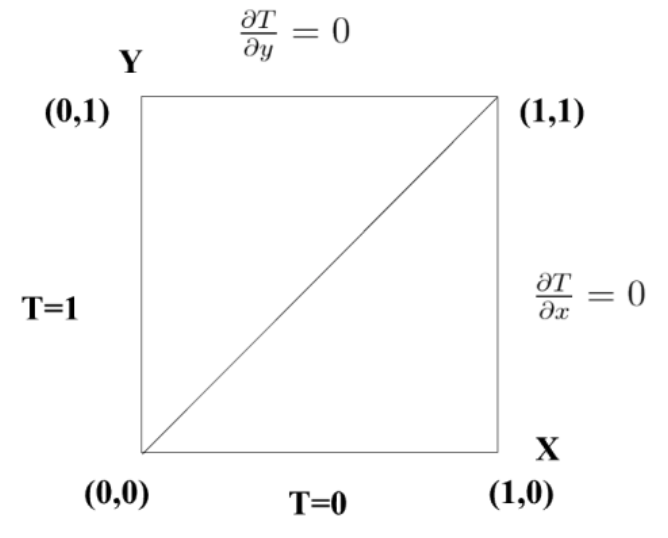
\includegraphics[width=0.5\textwidth]{10.png}
    \caption{Boundary Condition 2025 assignment 2}
    \label{fig:boundary}
\end{figure}
\noindent 具體邊界條件說明:

\noindent
\begin{minipage}[t]{0.5\textwidth} %[t]指得是頂部對齊 [b] 指的是底部對齊
   \begin{table}[H]
       \centering
       \renewcommand{\arraystretch}{1.8}
       \begin{tabular}{|c|c|c|}
           \hline
           \textbf{邊界位置} & \textbf{邊界條件類型} & \textbf{數學表達式} \\
            \hline
            左邊界 & Dirichlet & $T_{left} = 1$ \\
            \hline
            右邊界 & Dirichlet & $T_{right} = 0$ \\
            \hline
            上邊界 & Neumann & $\left.\frac{\partial T}{\partial y}\right|_{top}= 0$ \\
            \hline
            下邊界 & Dirichlet & $T_{bottom} = 0$ \\
            \hline
        \end{tabular}
        \label{tab:boundary}
    \end{table}
\end{minipage}
\hfill
\begin{minipage}[t]{0.5\textwidth}
    \begin{figure}[H]
        \centering
        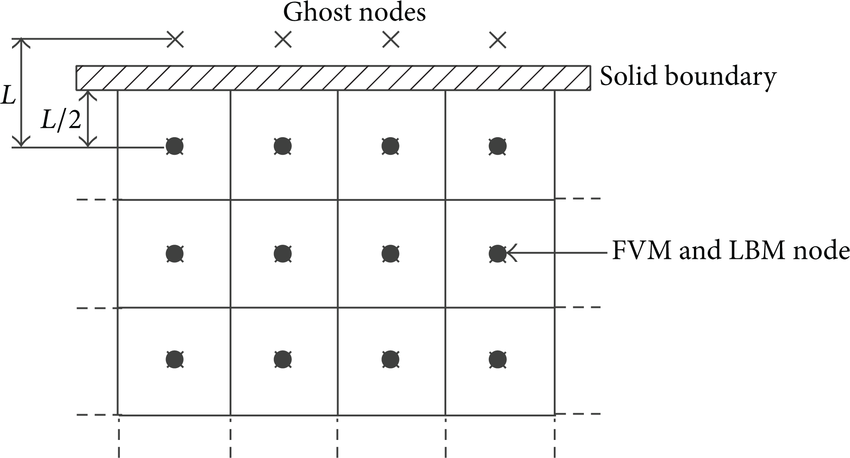
\includegraphics[width=\textwidth]{11.png}
        \caption{Link-Wise Bouundary}
        \label{fig:Link-Wise}
    \end{figure}
\end{minipage}\\[2.5ex]
\noindent 如圖\ref{fig:Link-Wise}所示,在有限體積法中,流場的離散定義域依據計算點的分佈,通常選定為Link-Wise Boundary,其特色為:(1)離散定義域的各個計算點為網格中心點,(2)離散定義域的邊界計算點與物理邊界相距半個網格空間。\\
\section{離散化方程式}
\begin{figure}[H]
        \centering
        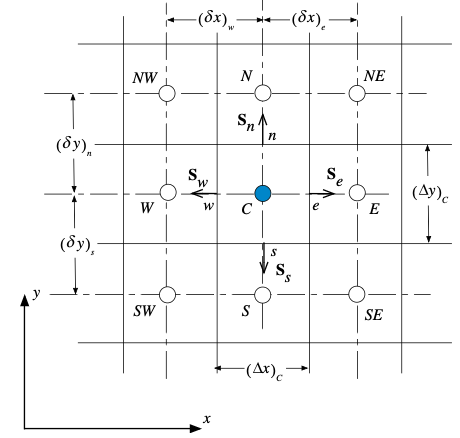
\includegraphics[width=0.3\textwidth]{12.png}
        \caption{FVM control volume}
        \label{fig:FVM_control_volume}
\end{figure}
\noindent 如圖\ref{fig:FVM_control_volume}所示,在有限體積法中,A流場的離散定義域選定為D Link-Wise Boundary,且對A流場的離散定義域的網格令為流體微元的控制體積,以建立守恆方程式。其中,需要注意的是,由於各個場的離散定義域的計算節點為離散定義域的網格中心點,對每一個網格建立方程式的過程中,需要差值代回網格中心點上的物理量取值。\\
\noindent 由式\eqref{eq:integration}出發,可以離散為
\begin{equation}\label{eq:discreete1}
    u_{e}T_{e}A_{e} - u_{w}T_{w}A_{w} + u_{n}T_{n}A_{n} - u_{s}T_{s}A_{s} = 0 \\
\end{equation}
\noindent 若A流場的離散定義域被定義為Link-Wise Boundary,則 在對離散定義域的網格建立守恆方程式的過程中,離散定義域的網格的邊界中心點的溫度,有如下處理:(以一維空間作為舉例)
\begin{equation}\begin{split}
    &\text{若}u_{e} > 0 , \text{則}T_{e} = \frac{6}{8}T_{P} + \frac{3}{8}T_{E} + \frac{-1}{8}T_{W} \\[1.5ex]
    &\text{若}u_{e} < 0 , \text{則}T_{e} = \frac{6}{8}T_{E} + \frac{3}{8}T_{P} + \frac{-1}{8}T_{EE} \\[1.5ex]
    &\text{若}u_{w} > 0 , \text{則}T_{w} = \frac{6}{8}T_{W} + \frac{3}{8}T_{P} + \frac{-1}{8}T_{WW} \\[1.5ex]
    &\text{若}u_{w} < 0 , \text{則}T_{w} = \frac{6}{8}T_{P} + \frac{3}{8}T_{W} + \frac{-1}{8}T_{E} \\[1.5ex]
\end{split}\end{equation}
上述取值即為QUICK離散格式的精髓,因此可以看出,QUICK離散格式是依附於「A流場的定義域為Link-Wise Bounfdary」的定義域計算點分佈。\\
若取(U(D穩態純對流方程)的(空間三階精度QUICK離散格式)),則上式\eqref{eq:discreete1}之離散格式可以進一步寫為:
\begin{equation}\label{QUICK1}\begin{split}
    &F_{e}(\frac{6}{8}T_{P} + \frac{3}{8}T_{E} + \frac{-1}{8}T_{W}) - F_{w}(\frac{6}{8}T_{W} + \frac{3}{8}T_{P} + \frac{-1}{8}T_{WW}) \\[1.5ex] 
    + &F_{n}(\frac{6}{8}T_{P} + \frac{3}{8}T_{N} + \frac{-1}{8}T_{S}) - F_{s}(\frac{6}{8}T_{S} + \frac{3}{8}T_{P} + \frac{-1}{8}T_{SS}) = 0 \\[1.5ex]
\end{split}\end{equation}
其中,\begin{equation}\begin{split}
    F_{e} = u_{e}A_{e}\ ;\ F_{w} = u_{w}A_{w}\ ;\ F_{n} = u_{n}A_{n}\ ;\ F_{s} = u_{s}A_{s} \\[1.5ex]
\end{split}\end{equation}
由於題目設定,在離散定義域的網格的邊界中心點上,皆有$u_{e} = 1.0\ ;\ u_{w} = 1.0$,且離散定義域為正方網格系統,因此對於離散定義域的網格,也有:$A_{e} = A_{w} = A_{n} = A_{s}$
,故對於離散定義域的內網格,有:
\begin{equation}\label{eq:innerQUICK}\begin{split}
   &\Delta y (\frac{3}{8}T_{E} + \frac{3}{8}T_{P} +  \frac{-7}{8}T_{W}+ \frac{1}{8}T_{WW}) \\[1.5ex]
   +& \Delta x (\frac{3}{8}T_{N} + \frac{3}{8}T_{P} +  \frac{-7}{8}T_{S}+ \frac{1}{8}T_{SS}) = 0 \\[1.5ex]
\end{split}\end{equation}
上式即為A流場的離散定義域中,(E(I(S內計算點)的(穩態純對流方程))的(空間三階精度QUICK離散格式))
\section{邊界處理}
在二維空間中,且離散格式取QUICK離散格式下,原則上需要對於六個邊界、九個角點特別討論其上的離散方程。
\begin{figure}[H]
        \centering
        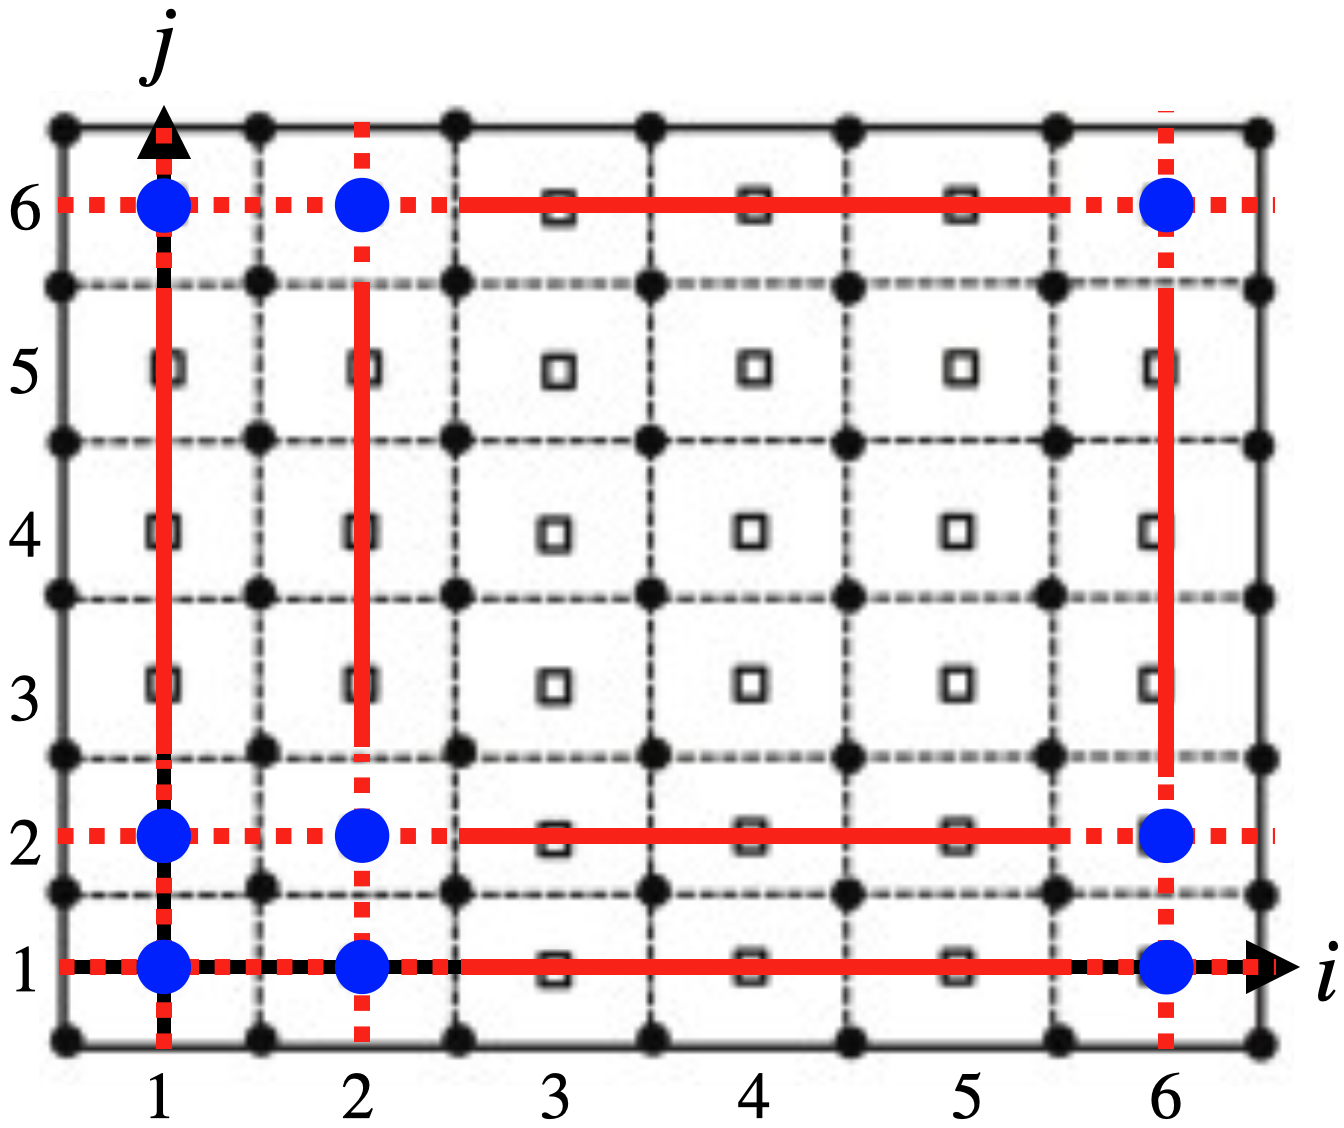
\includegraphics[width=0.5\textwidth]{13.png}
        \caption{Illustration of the QUICK scheme: handling six boundaries and nine corner points}
        \label{fig:QUICK_scheme_boundaries}
\end{figure}
\noindent 下面依序討論各個邊界點所應該滿足的離散化方程(各個邊界點的(E(W(R穩態純對流方程)的(積分形式))的(空間三階精度QUICK離散格式)))。

\subsection{左邊界計算點}
 \begin{minipage}{0.6\textwidth}
   \noindent 範圍:$i=1\ ,\ j\in[3\ ,\ N_{y}-1]$\\[1.5ex]
   \noindent 邊界條件:$T_{left} = T_{-\frac{1}{2},j}= 1$\\[1.5ex]
   \noindent 空間三階精度QUICK離散格式為:
   \begin{equation*}\label{eq:QUICK1}\begin{split}
    &\Delta y(\frac{3}{8}T_{2,j} + \frac{7}{8}T_{1,j})\\[1.5ex]
    +& \Delta x (\frac{3}{8}T_{1,j+1} + \frac{3}{8}T_{1,j} +  \frac{-7}{8}T_{1,j-1}+ \frac{1}{8}T_{1,j-2}) = \Delta y\frac{10}{8}T_{left} \\
   \end{split}\end{equation*}
   \end{minipage}%
   \hfill
   \begin{minipage}{0.34\textwidth}
   \centering
   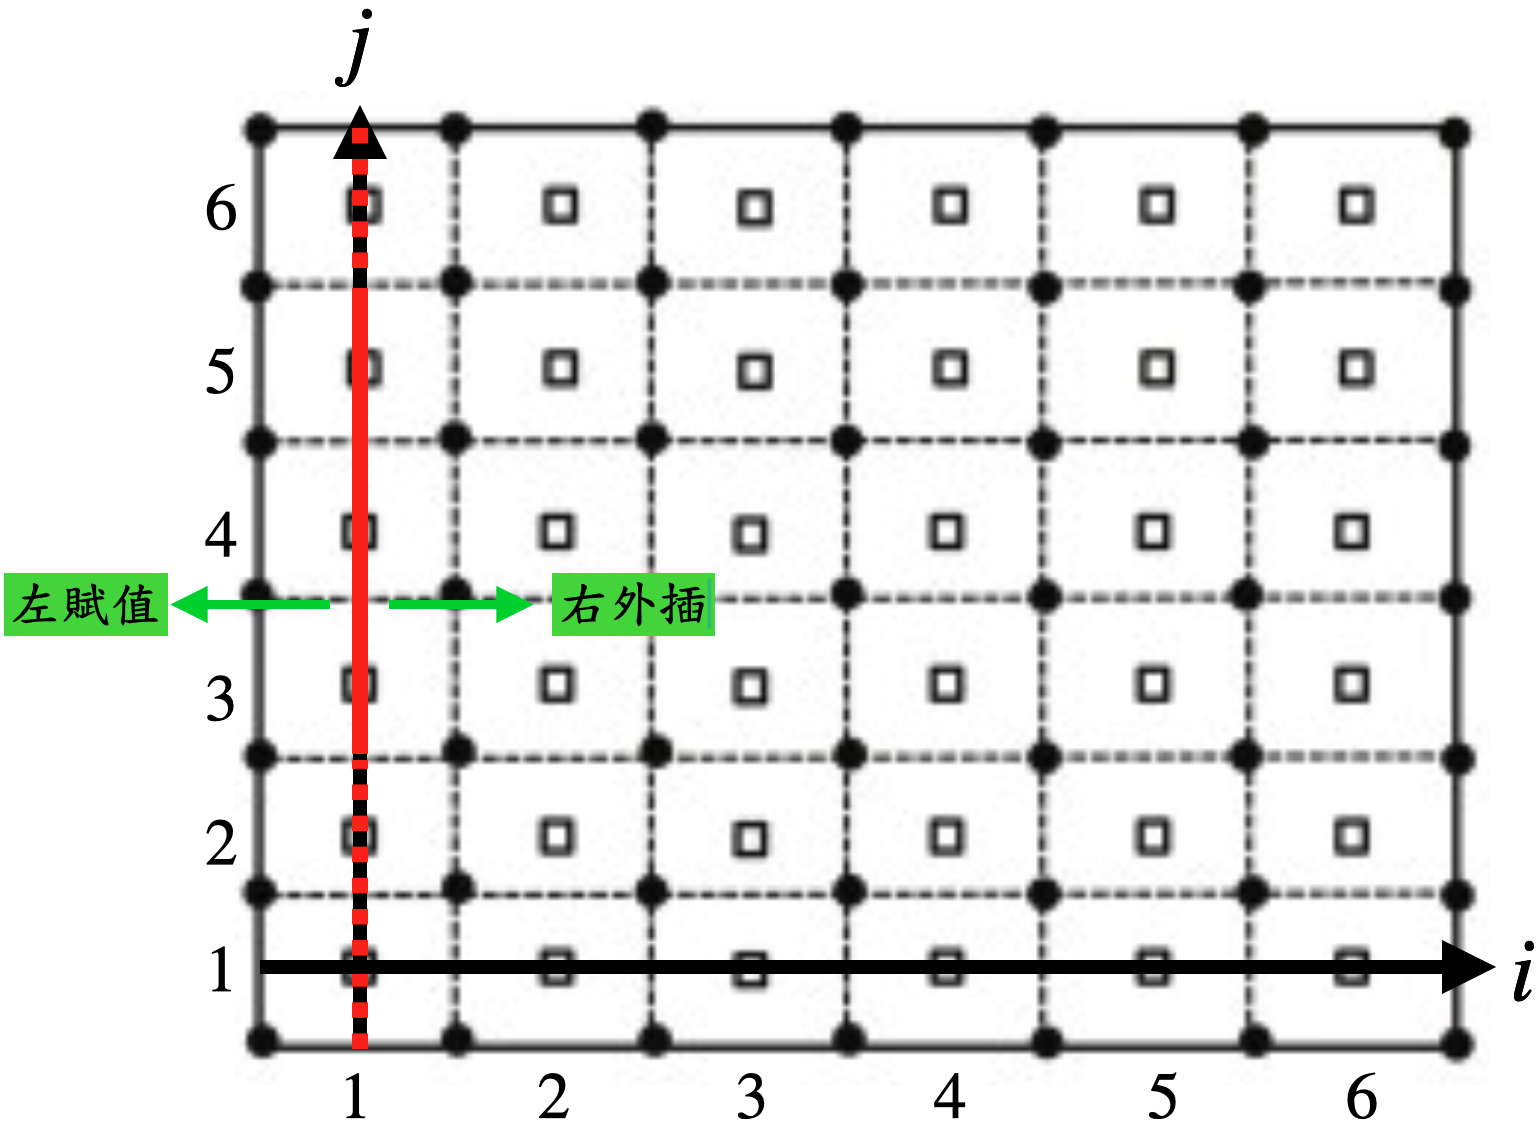
\includegraphics[width=\linewidth,height=9\baselineskip]{14.png}
   \label{fig:1boundary}
\end{minipage}
\subsection{右邊界計算點}
 \begin{minipage}{0.6\textwidth}
   \noindent 範圍:$i=N_{x}\ ,\ j\in[3\ ,\ N_{y}-1]$\\[1.5ex]
   \noindent 邊界條件:$T_{right} = T_{N_{x}+\frac{1}{2},j}= 0$\\[1.5ex]
   \noindent 空間三階精度QUICK離散格式為:
   \begin{equation*}\label{eq:QUICK2}\begin{split}
   -&\Delta y(\frac{3}{8}T_{N_{x},j} + \frac{6}{8}T_{N_{x}-1,j} + \frac{-1}{8}T_{N_{x}-2,j}) \\[1.5ex] 
   +& \Delta x (\frac{3}{8}T_{N_{x},j+1} + \frac{3}{8}T_{N_{x},j} +  \frac{-7}{8}T_{N_{x},j-1}+ \frac{1}{8}T_{N_{x},j-2}) = -\Delta y T_{right} \\[1.5ex]
   \end{split}\end{equation*}
   \end{minipage}%
   \hfill
   \begin{minipage}{0.34\textwidth}
   \centering
   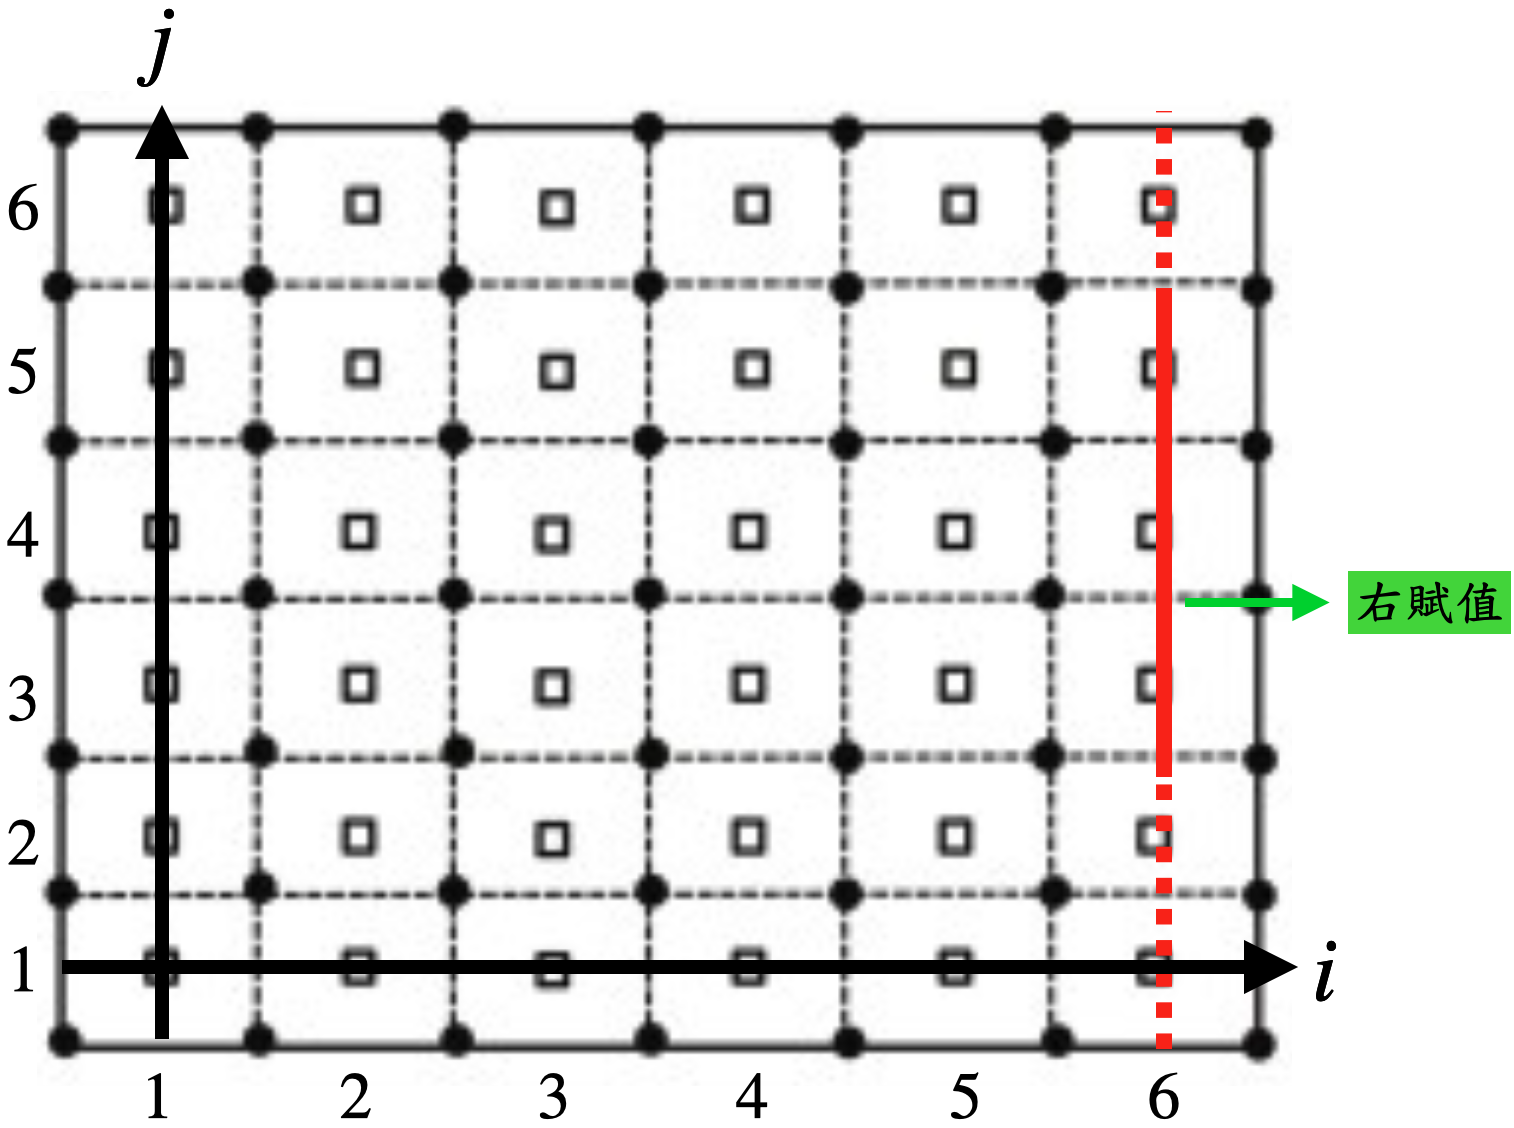
\includegraphics[width=\linewidth,height=9\baselineskip]{15.png}
   \label{fig:2boundary}
\end{minipage}

\subsection{下邊界計算點}
 \begin{minipage}{0.6\textwidth}
   \noindent 範圍:$i\in[3\ ,\ N_{x}-1]\ ,\ j=1$\\[1.5ex]
   \noindent 邊界條件:$T_{bottom} = T_{i,-\frac{1}{2}}= 0$\\[1.5ex]
   \noindent 空間三階精度QUICK離散格式為:
   \begin{equation*}\label{eq:QUICK3}\begin{split}
      &\Delta y (\frac{3}{8}T_{i+1,1} + \frac{3}{8}T_{i,1} +  \frac{-7}{8}T_{i-1,1}+ \frac{1}{8}T_{i-2,1}) \\[1.5ex]
    + &\Delta x (\frac{3}{8}T_{i,2} + \frac{7}{8}T_{i,1} ) =\Delta x\frac{10}{8}T_{bottom} \\[1.5ex]
   \end{split}\end{equation*}
   \end{minipage}%
   \hfill
   \begin{minipage}{0.34\textwidth}
   \centering
   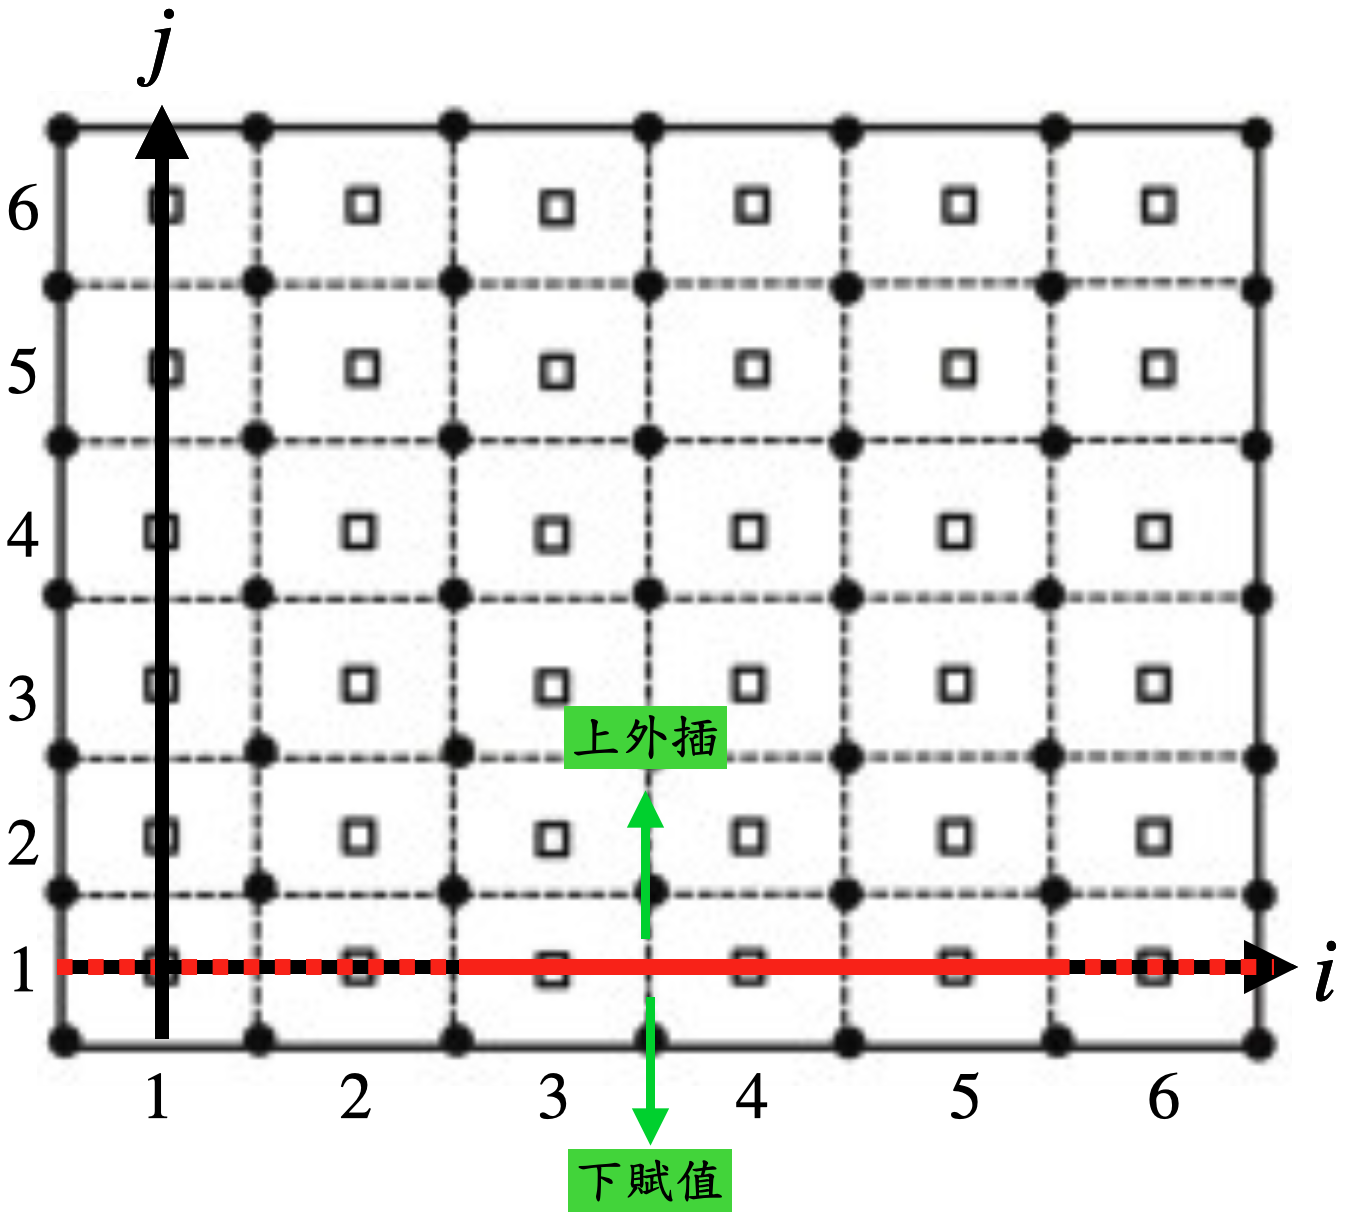
\includegraphics[width=\linewidth,height=9\baselineskip]{16.png}
   \label{fig:3boundary}
\end{minipage}
\subsection{上邊界計算點}
 \begin{minipage}{0.6\textwidth}
    \noindent 範圍:$i\in[3\ ,\ N_{x}-1]\ ,\ j=N_{y}$\\[1.5ex]
   \noindent 邊界條件:$T_{up} = T_{1,N_{y}+\frac{1}{2}}=T_{1,N_{y}-\frac{1}{2}}$\\[1.5ex]
   \noindent 空間三階精度QUICK離散格式為:
   \begin{equation*}\label{eq:QUICK4}\begin{split}
    \Delta y (\frac{3}{8}T_{i+1,N_{y}} + \frac{3}{8}T_{i,N_{y}} +  \frac{-7}{8}T_{i-1,N_{y}}+ \frac{1}{8}T_{i-2,N_{y}}) = 0 \\[1.5ex]
   \end{split}\end{equation*}
   \end{minipage}%
   \hfill
   \begin{minipage}{0.34\textwidth}
   \centering
   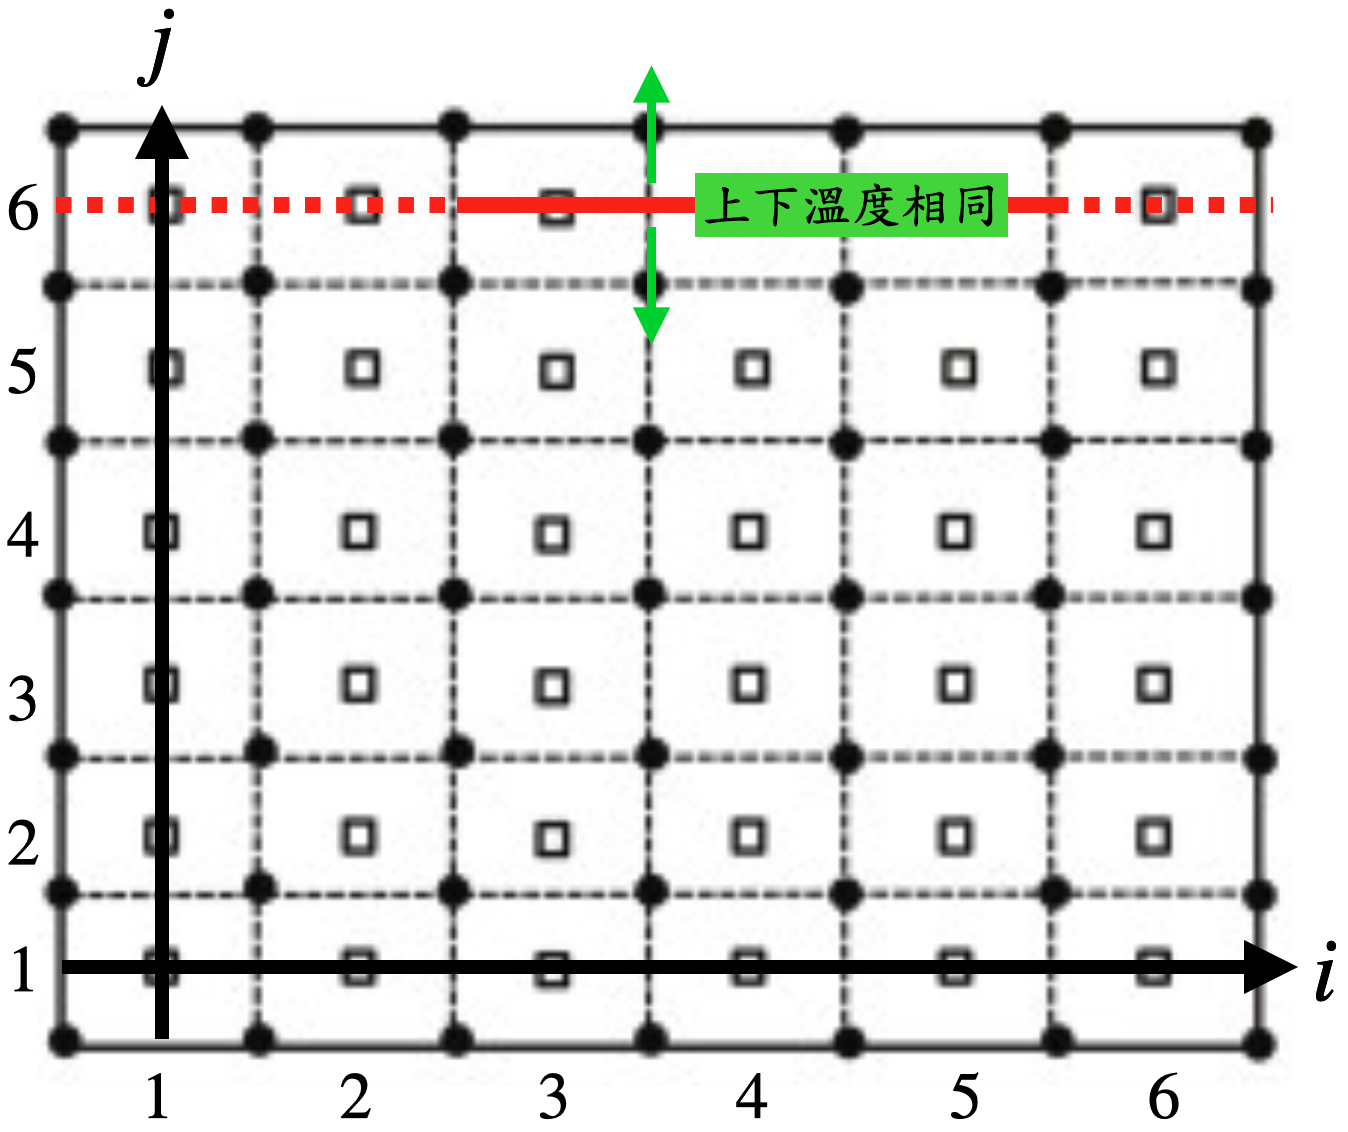
\includegraphics[width=\linewidth,height=9\baselineskip]{17.png}
   \label{fig:4boundary}
\end{minipage}

\subsection{左第二排邊界計算點}
 \begin{minipage}{0.6\textwidth}
   \noindent 範圍:$i=2\ ,\ j\in[3\ ,\ N_{y}-1]$\\[1.5ex]
   \noindent 邊界條件:$T_{left} = T_{-\frac{1}{2},j}= 1$\\[1.5ex]
   \noindent 空間三階精度QUICK離散格式為:
   \begin{equation*}\label{eq:QUICK5}\begin{split}
     &\Delta y(\frac{3}{8}T_{3,j} + \frac{3}{8}T_{2,j} -T_{1,j})\\[1.5ex] 
    +& \Delta x (\frac{3}{8}T_{2,j+1} + \frac{3}{8}T_{2,j} +  \frac{-7}{8}T_{2,j-1}+ \frac{1}{8}T_{2,j-2}) =\Delta y \frac{-2}{8}(T_{left}) \\[1.5ex]
   \end{split}\end{equation*}
   \end{minipage}%
   \hfill
   \begin{minipage}{0.34\textwidth}
   \centering
   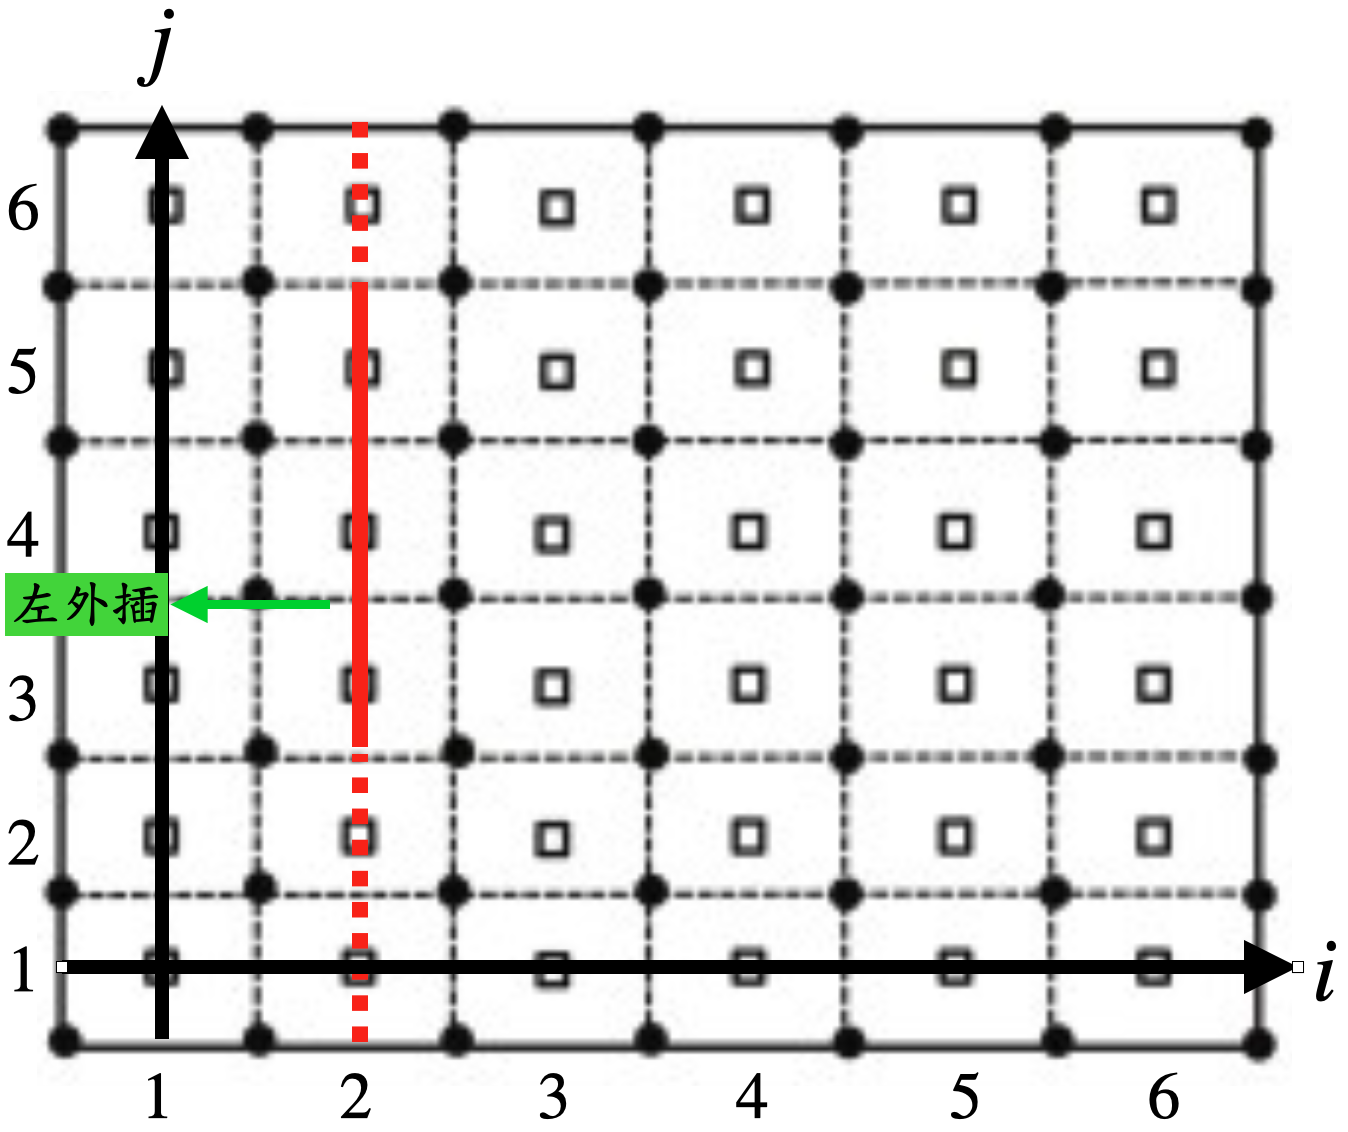
\includegraphics[width=\linewidth,height=9\baselineskip]{18.png}
   \label{fig:5boundary}
\end{minipage}
\subsection{下第二排邊界計算點}
 \begin{minipage}{0.6\textwidth}
   \noindent 範圍:$i\in[3\ ,\ N_{x}-1]\ ,\ j=2$\\[1.5ex]
   \noindent 邊界條件:$T_{bottom} = T_{i,-\frac{1}{2}}= 0$\\[1.5ex]
   \noindent 空間三階精度QUICK離散格式為:
   \begin{equation*}\label{eq:QUICK6}\begin{split}
      &\Delta y (\frac{3}{8}T_{i+1,2} + \frac{3}{8}T_{i,2} +  \frac{-7}{8}T_{i-1,2}+ \frac{1}{8}T_{i-2,2}) \\[1.5ex]
    + &\Delta x(\frac{3}{8}T_{i,3} + \frac{3}{8}T_{i,2} - T_{i,1}) =  \Delta x\frac{-2}{8}T_{bottom} \\[1.5ex]
   \end{split}\end{equation*}
   \end{minipage}%                          
   \hfill
   \begin{minipage}{0.34\textwidth}
   \centering
   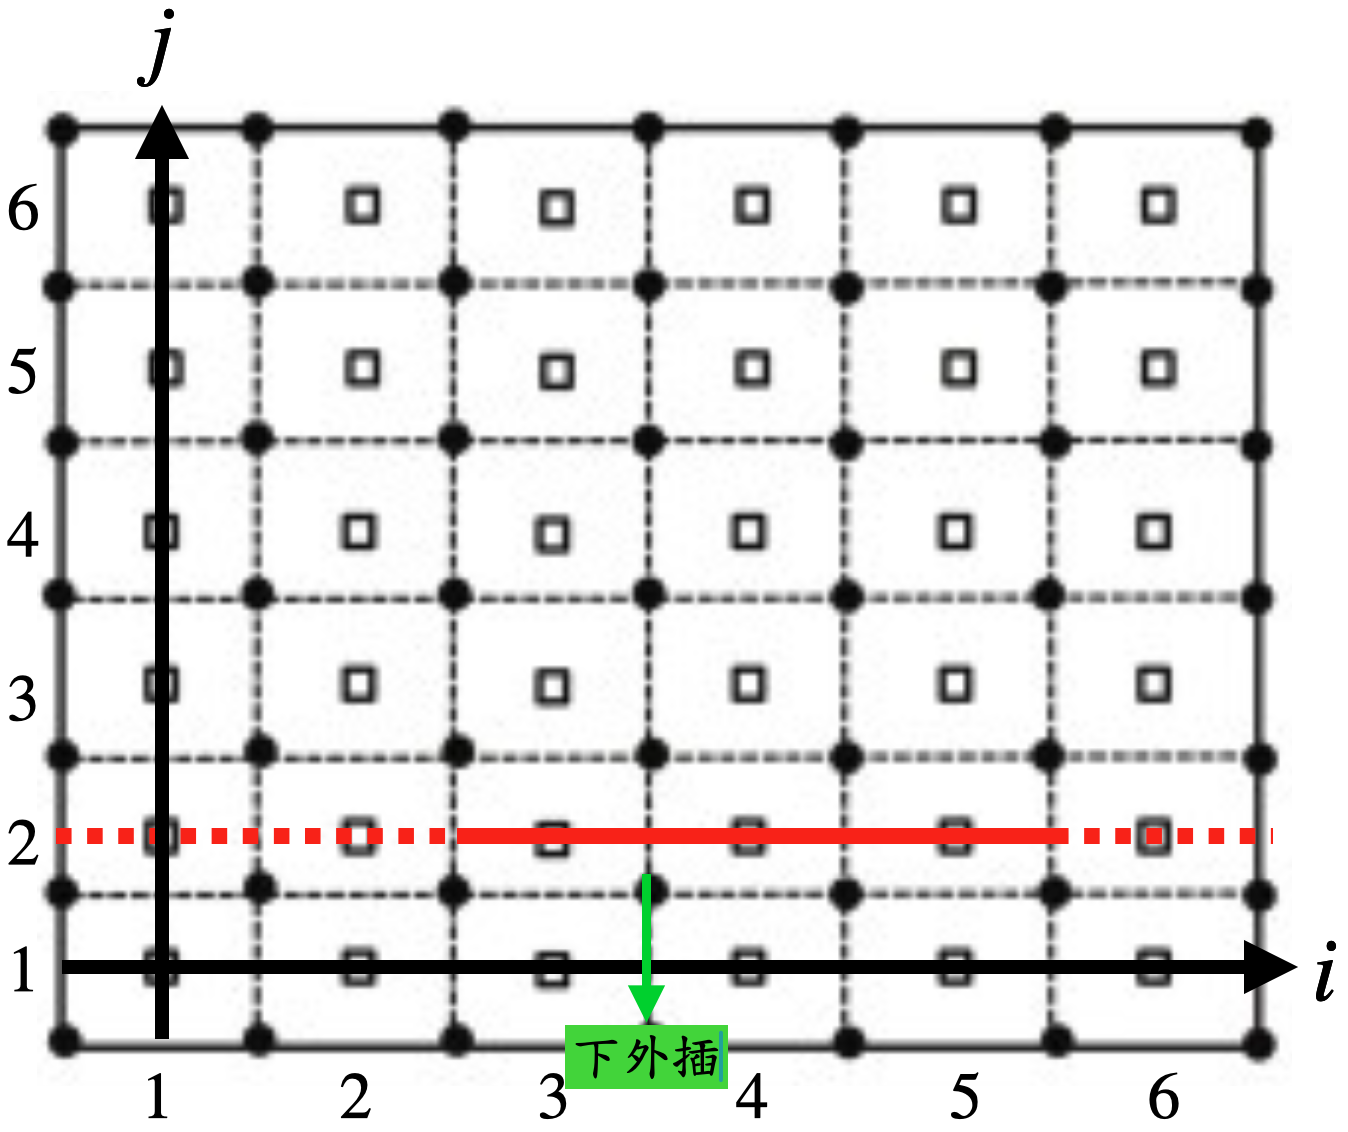
\includegraphics[width=\linewidth,height=9\baselineskip]{19.png}
   \label{fig:6boundary}
\end{minipage}
\section{角點處理}
\noindent 在空間三階精度QUICK離散格式中,一維離散定義域的三個節點需要特別處理,二維離散定義域的九個角點需要特別處理。根據題目得設定,在離散定義域的網格的邊界中心點的速度場,皆有$u_{e},u_{w}>0$,因此,九個需要特別處理的計算點呈現如下分佈。\\
\subsection{第一計算點}
 \begin{minipage}{0.6\textwidth}
   \noindent 範圍:$i=1\ ,\ i=1$\\[1.5ex]
   \noindent 邊界條件:$T_{left} = T_{-\frac{1}{2},1}= 1\ ,\ T_{botttom} = T_{1,-\frac{1}{2}}= 0$\\[1.5ex]
   \noindent 東西方向:採用式\eqref{eq:QUICK1}$\ ,\ $南北方向:採用式\eqref{eq:QUICK3}\\[1.5ex]
   \noindent 空間三階精度QUICK離散格式為:
   \begin{equation*}\begin{split}
    &\Delta y(\frac{3}{8}T_{2,1} + \frac{7}{8}T_{1,1})\\[1.5ex]
   +&\Delta x (\frac{3}{8}T_{1,2} + \frac{7}{8}T_{1,1} ) = \Delta y\frac{10}{8}T_{left}+\Delta x\frac{10}{8}T_{bottom} \\[1.5ex]
   \end{split}\end{equation*}
   \end{minipage}%
   \hfill
   \begin{minipage}{0.34\textwidth}
   \centering
   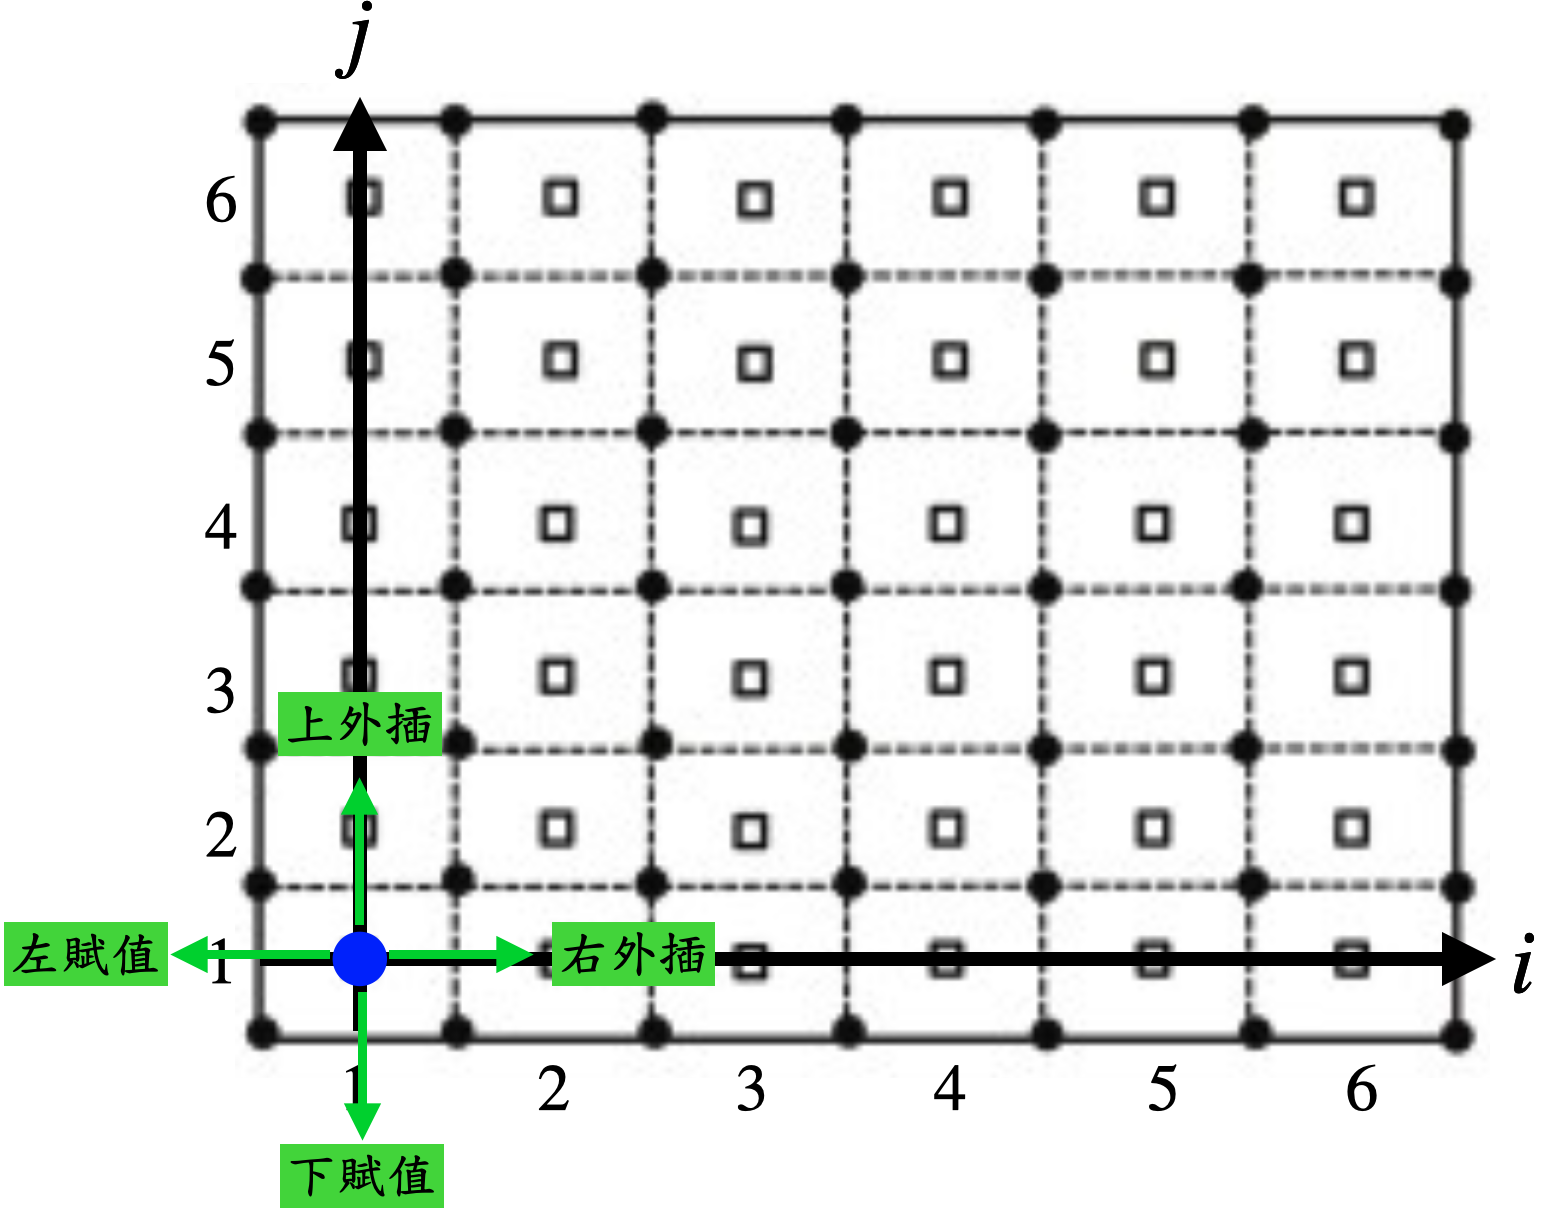
\includegraphics[width=\linewidth,height=9\baselineskip]{20.png}
   \label{fig:1st point}
\end{minipage}
\subsection{第二計算點}
 \begin{minipage}{0.6\textwidth}
   \noindent 範圍:$i=2\ ,\ j=1$\\[1.5ex]
   \noindent 邊界條件:$T_{left} = T_{-\frac{1}{2},1}= 1\ ,\ T_{botttom} = T_{2,-\frac{1}{2}}= 0$\\[1.5ex]
   \noindent 東西方向:採用式\eqref{eq:QUICK5}$\ ,\ $南北方向:採用式\eqref{eq:QUICK3}\\[1.5ex]
   \noindent 空間三階精度QUICK離散格式為:
   \begin{equation*}\begin{split}
   &\Delta y(\frac{3}{8}T_{3,1} + \frac{3}{8}T_{2,1} -T_{1,1})\\[1.5ex] 
  +&\Delta x (\frac{3}{8}T_{2,2} + \frac{7}{8}T_{2,1} ) =\Delta y \frac{-2}{8}(T_{left})+\Delta x\frac{10}{8}T_{bottom} \\[1.5ex] 
   \end{split}\end{equation*}
   \end{minipage}                          
   \hfill
   \begin{minipage}{0.34\textwidth}
   \centering
   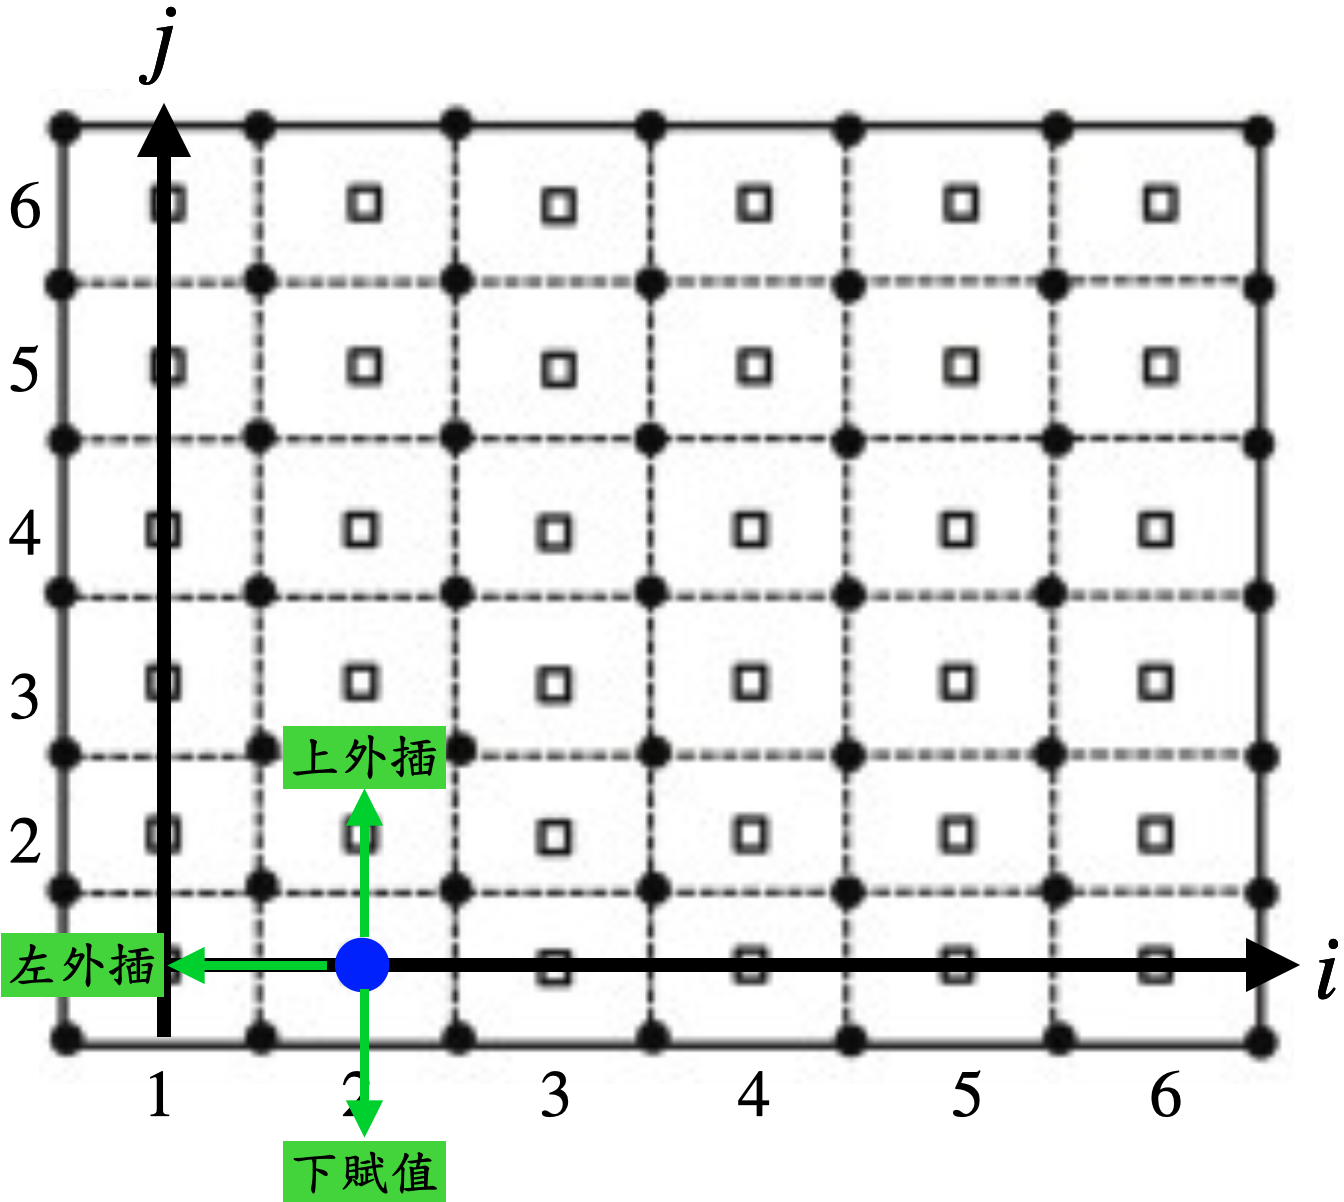
\includegraphics[width=\linewidth,height=9\baselineskip]{21.png}
   \label{fig:2nd point}
\end{minipage}
\subsection{第三計算點}
 \begin{minipage}{0.6\textwidth}
   \noindent 範圍:$i=N_{x}\ ,\ j=1$\\[1.5ex]
   \noindent 邊界條件:$T_{right} = T_{N_{x}+\frac{1}{2},1}= 0\ ,\ T_{botttom} = T_{N_{x},-\frac{1}{2}}= 0$\\[1.5ex]
   \noindent 東西方向:採用式\eqref{eq:QUICK2}$\ ,\ $南北方向:採用式\eqref{eq:QUICK3}\\[1.5ex]
   \noindent 空間三階精度QUICK離散格式為:
   \begin{equation*}\begin{split}
   -&\Delta y(\frac{3}{8}T_{N_{x},1} + \frac{6}{8}T_{N_{x}-1,1} + \frac{-1}{8}T_{N_{x}-2,1}) \\[1.5ex] 
   +&\Delta x (\frac{3}{8}T_{N_{x},2} + \frac{7}{8}T_{N_{x},1} ) = -\Delta y T_{right} + \Delta x\frac{10}{8}T_{bottom} \\[1.5ex]
   \end{split}\end{equation*}
   \end{minipage}%
   \hfill
   \begin{minipage}{0.34\textwidth}
   \centering
   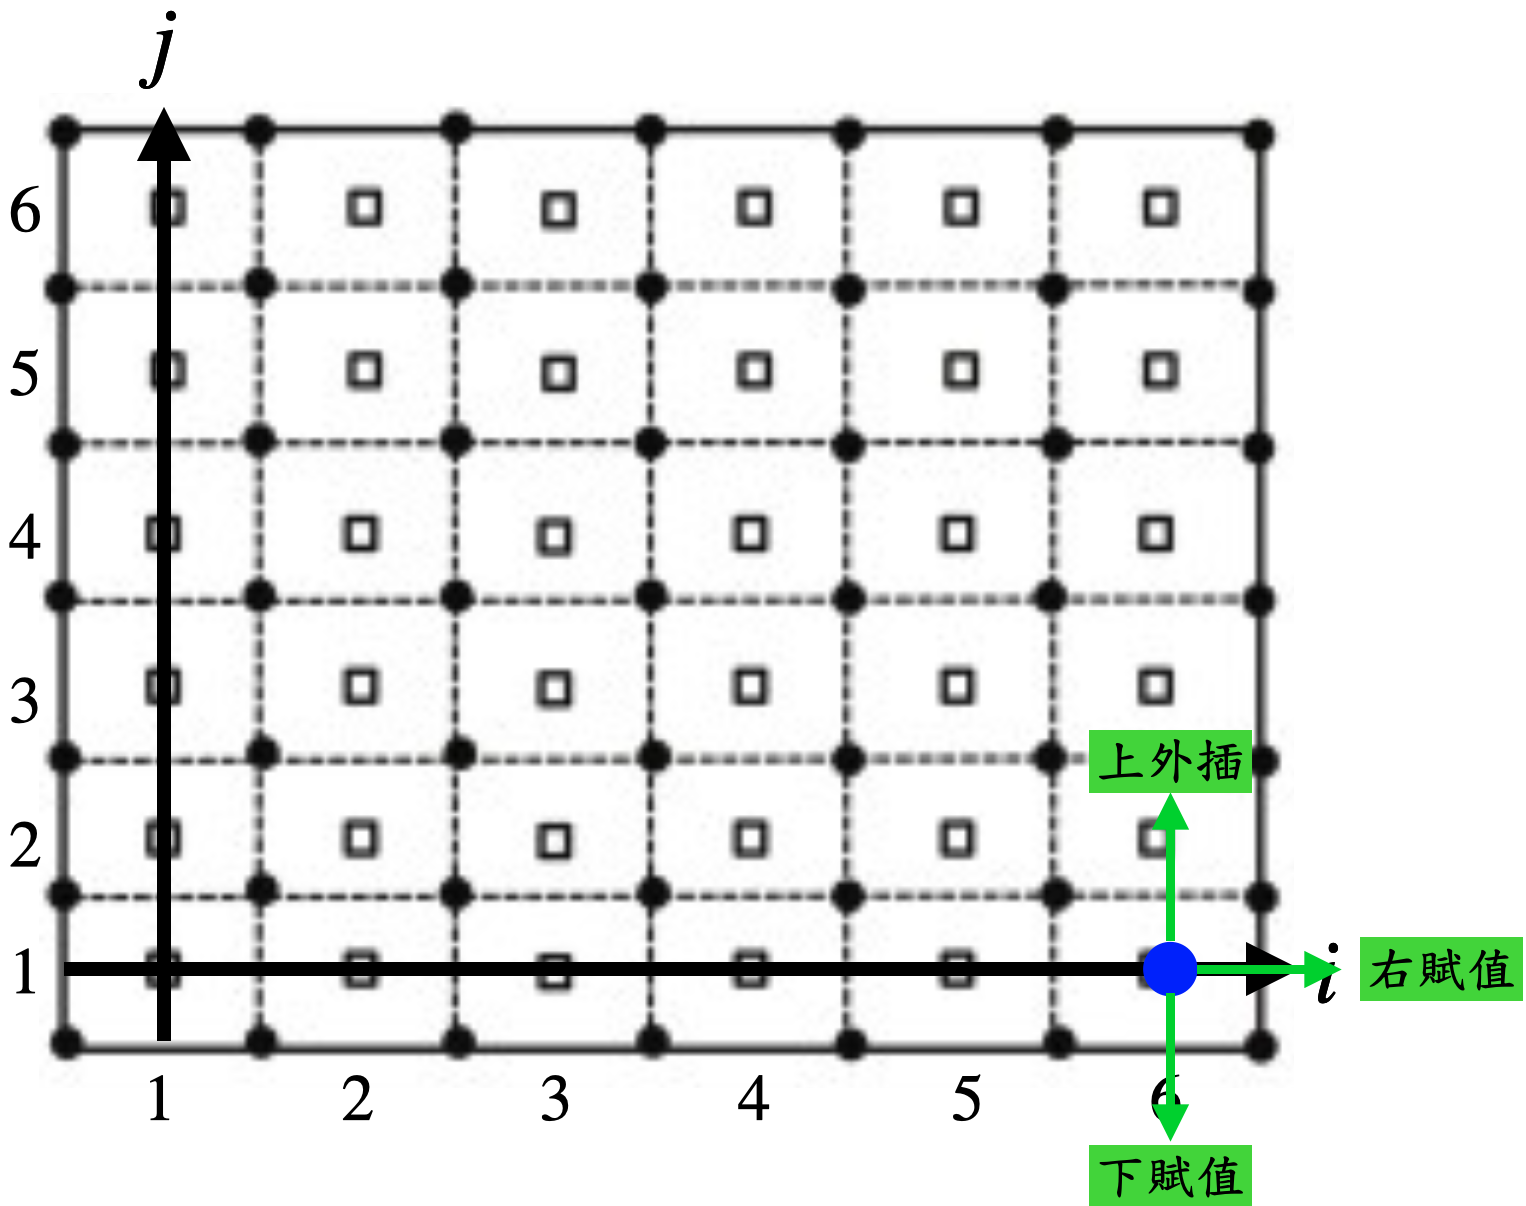
\includegraphics[width=\linewidth,height=9\baselineskip]{22.png}
   \label{fig:3rd point}
\end{minipage}



\subsection{第四計算點}
 \begin{minipage}{0.6\textwidth}
   \noindent 範圍:$i=1\ ,\ i=2$\\[1.5ex]
   \noindent 邊界條件:$T_{left} = T_{-\frac{1}{2},2}= 1\ ,\ T_{botttom} = T_{1,-\frac{1}{2}}= 0$\\[1.5ex]
   \noindent 東西方向:採用式\eqref{eq:QUICK1}$\ ,\ $南北方向:採用式\eqref{eq:QUICK6}\\[1.5ex]
   \noindent 空間三階精度QUICK離散格式為:
   \begin{equation*}\begin{split}
    &\Delta y(\frac{3}{8}T_{2,2} + \frac{7}{8}T_{1,2})\\[1.5ex]
   +&\Delta x(\frac{3}{8}T_{1,3} + \frac{3}{8}T_{1,2} - T_{1,1}) = \Delta y\frac{10}{8}T_{left} + \Delta x\frac{-2}{8}T_{bottom}\\
   \end{split}\end{equation*}
   \end{minipage}%
   \hfill
   \begin{minipage}{0.34\textwidth}
   \centering
   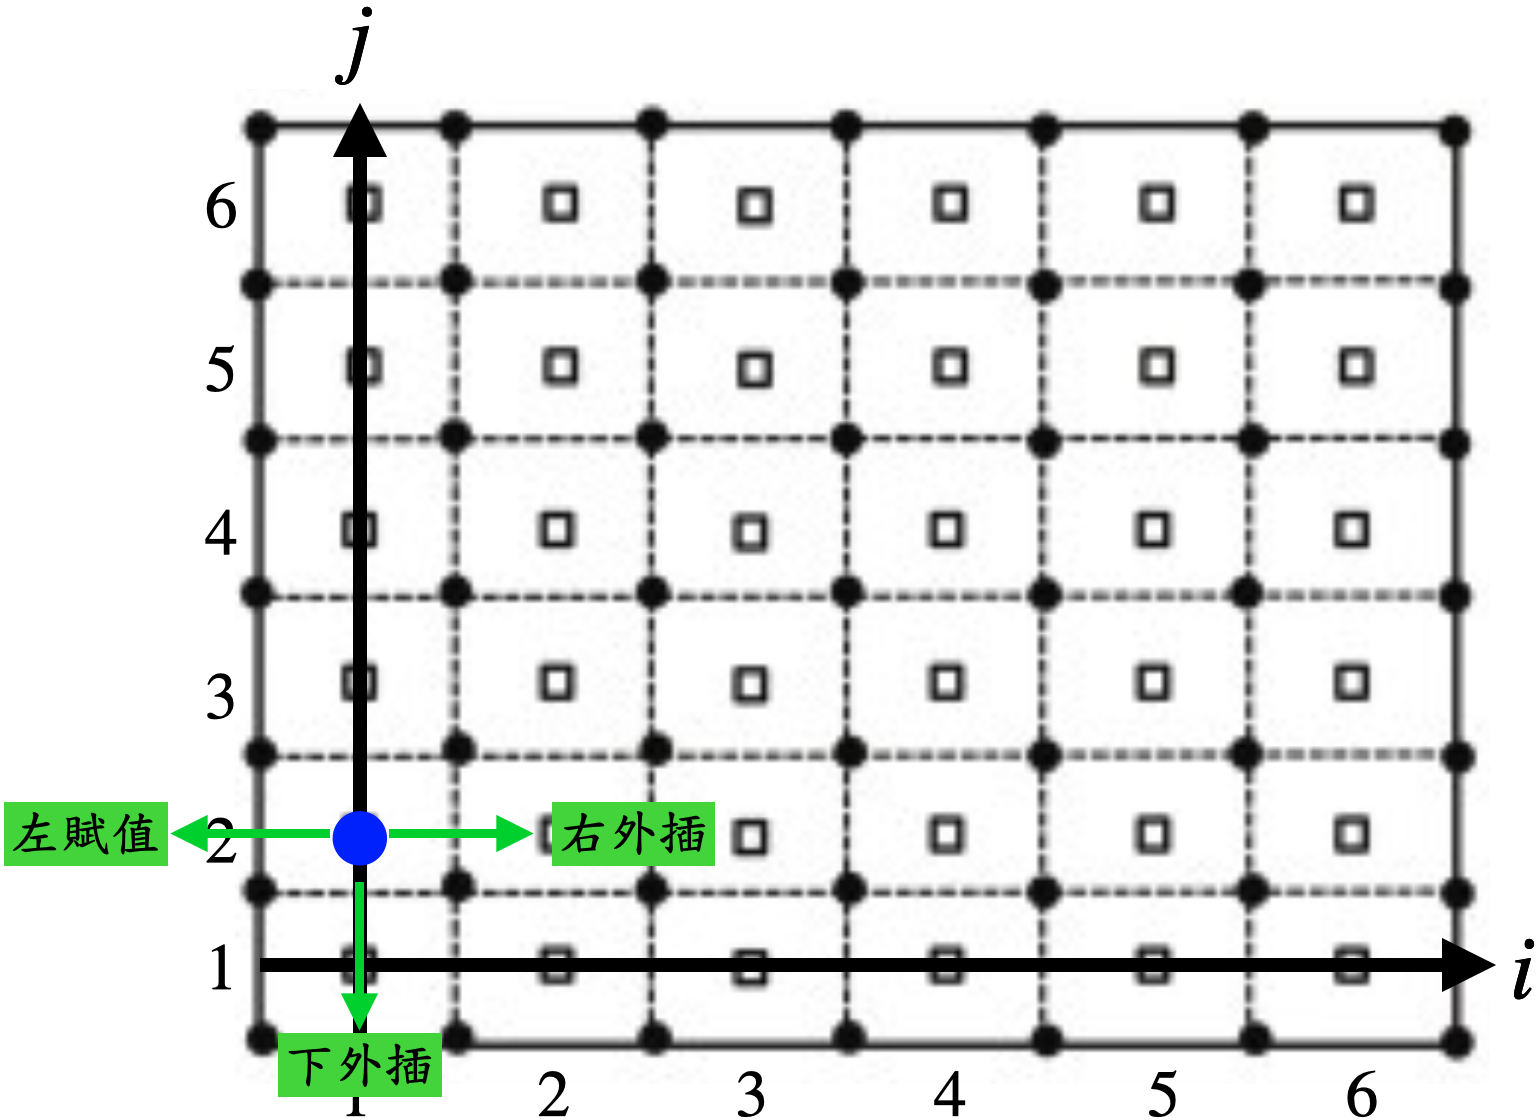
\includegraphics[width=\linewidth,height=9\baselineskip]{23.png}
   \label{fig:4th point}
\end{minipage}
\subsection{第五計算點}
 \begin{minipage}{0.6\textwidth}
   \noindent 範圍:$i=2\ ,\ j=2$\\[1.5ex]
   \noindent 邊界條件:$T_{left} = T_{-\frac{1}{2},2}= 1\ ,\ T_{botttom} = T_{2,-\frac{1}{2}}= 0$\\[1.5ex]
   \noindent 東西方向:採用式\eqref{eq:QUICK5}$\ ,\ $南北方向:採用式\eqref{eq:QUICK6}\\[1.5ex]
   \noindent 空間三階精度QUICK離散格式為:
   \begin{equation*}\begin{split}
   &\Delta y(\frac{3}{8}T_{3,2} + \frac{3}{8}T_{2,2} -T_{1,2})\\[1.5ex] 
  +&\Delta x(\frac{3}{8}T_{2,3} + \frac{3}{8}T_{2,2} - T_{2,1}) =\Delta y \frac{-2}{8}(T_{left}) + \Delta x\frac{-2}{8}T_{bottom} \\[1.5ex]
   \end{split}\end{equation*}
   \end{minipage}                          
   \hfill
   \begin{minipage}{0.34\textwidth}
   \centering
   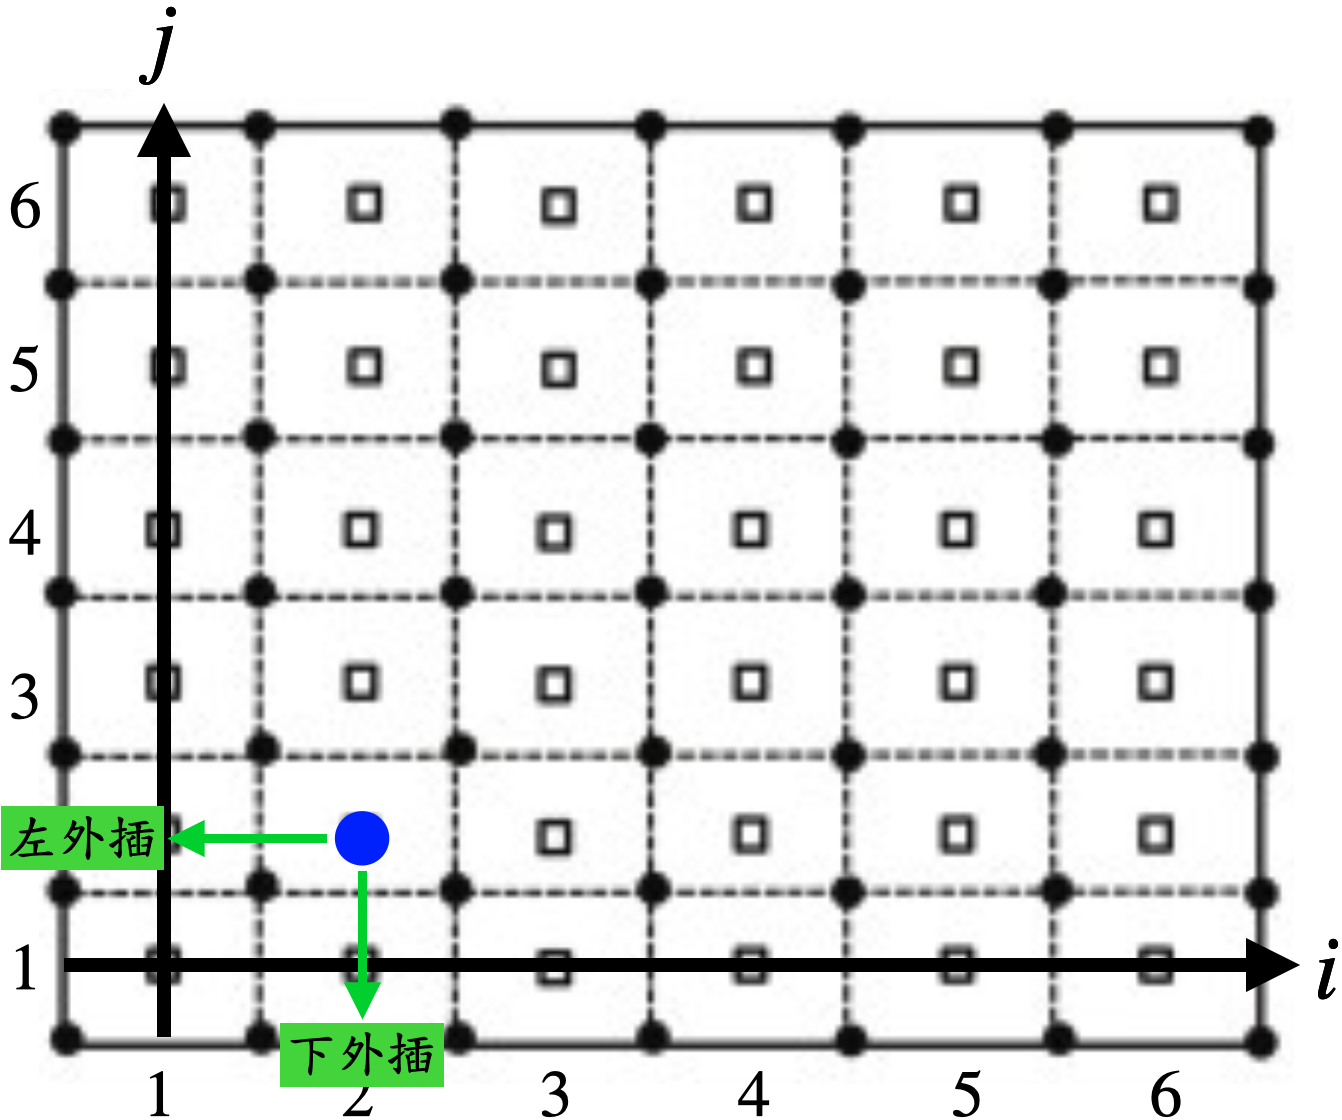
\includegraphics[width=\linewidth,height=9\baselineskip]{24.png}
   \label{fig:5th point}
\end{minipage}
\subsection{第六計算點}
 \begin{minipage}{0.6\textwidth}
   \noindent 範圍:$i=N_{x}\ ,\ j=2$\\[1.5ex]
   \noindent 邊界條件:$T_{right} = T_{N_{x}+\frac{1}{2},2}= 0\ ,\ T_{botttom} = T_{N_{x},-\frac{1}{2}}= 0$\\[1.5ex]
   \noindent 東西方向:採用式\eqref{eq:QUICK2}$\ ,\ $南北方向:採用式\eqref{eq:QUICK6}\\[1.5ex]
   \noindent 空間三階精度QUICK離散格式為:
   \begin{equation*}\begin{split}
   - &\Delta y(\frac{3}{8}T_{N_{x},2} + \frac{6}{8}T_{N_{x}-1,2} + \frac{-1}{8}T_{N_{x}-2,2}) \\[1.5ex] 
   + &\Delta x(\frac{3}{8}T_{N_{x},3} + \frac{3}{8}T_{N_{x},2} - T_{N_{x},1}) =  -\Delta y T_{right}+\Delta x\frac{-2}{8}T_{bottom} \\[1.5ex]
   \end{split}\end{equation*}
   \end{minipage}%
   \hfill
   \begin{minipage}{0.34\textwidth}
   \centering
   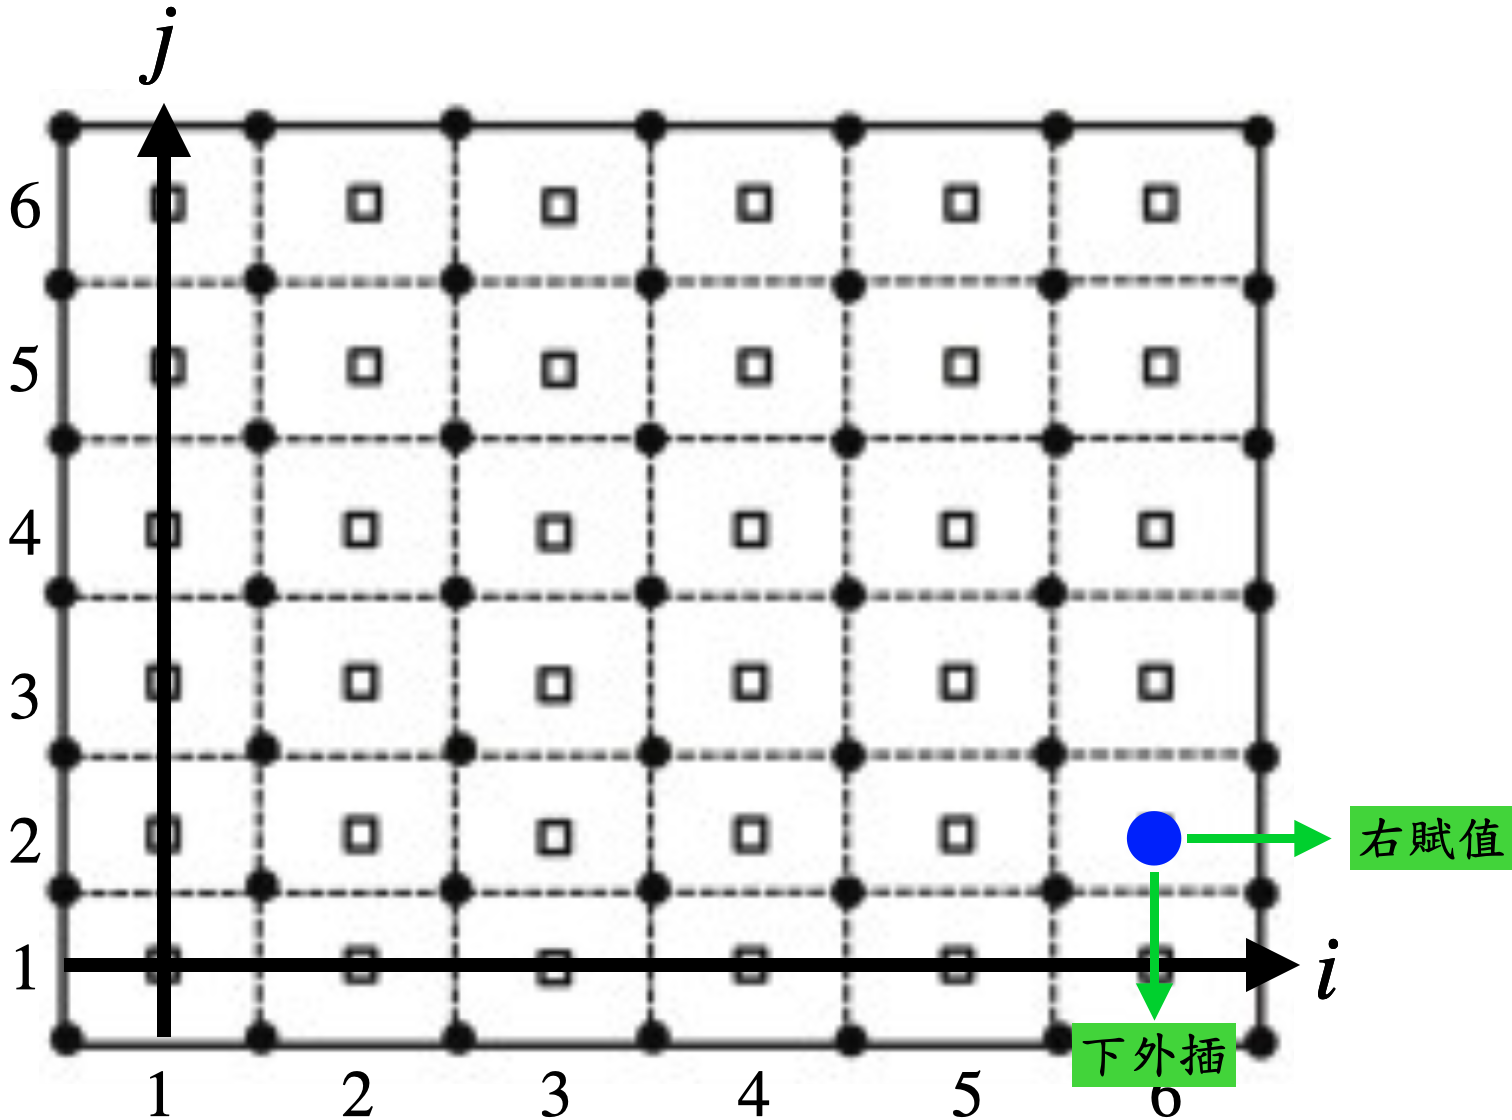
\includegraphics[width=\linewidth,height=9\baselineskip]{25.png}
   \label{fig:6th point}
\end{minipage}








\newpage
\subsection{第七計算點}
 \begin{minipage}{0.6\textwidth}
   \noindent 範圍:$i=1\ ,\ j=N_{y}$\\[1.5ex]
   \noindent 邊界條件:$T_{left} = T_{-\frac{1}{2},N_{y}}= 1\ ,\ T_{up} = T_{1,N_{y}+\frac{1}{2}}=T_{1,N_{y}-\frac{1}{2}}$\\[1.5ex]
   \noindent 東西方向:採用式\eqref{eq:QUICK1}$\ ,\ $南北方向:採用式\eqref{eq:QUICK4}\\[1.5ex]
   \noindent 空間三階精度QUICK離散格式為:
   \begin{equation*}\begin{split}
   \Delta y(\frac{3}{8}T_{2,j} + \frac{7}{8}T_{1,j}) = \Delta y\frac{10}{8}T_{left} \\
   \end{split}\end{equation*}
   \end{minipage}%
   \hfill
   \begin{minipage}{0.34\textwidth}
   \centering
   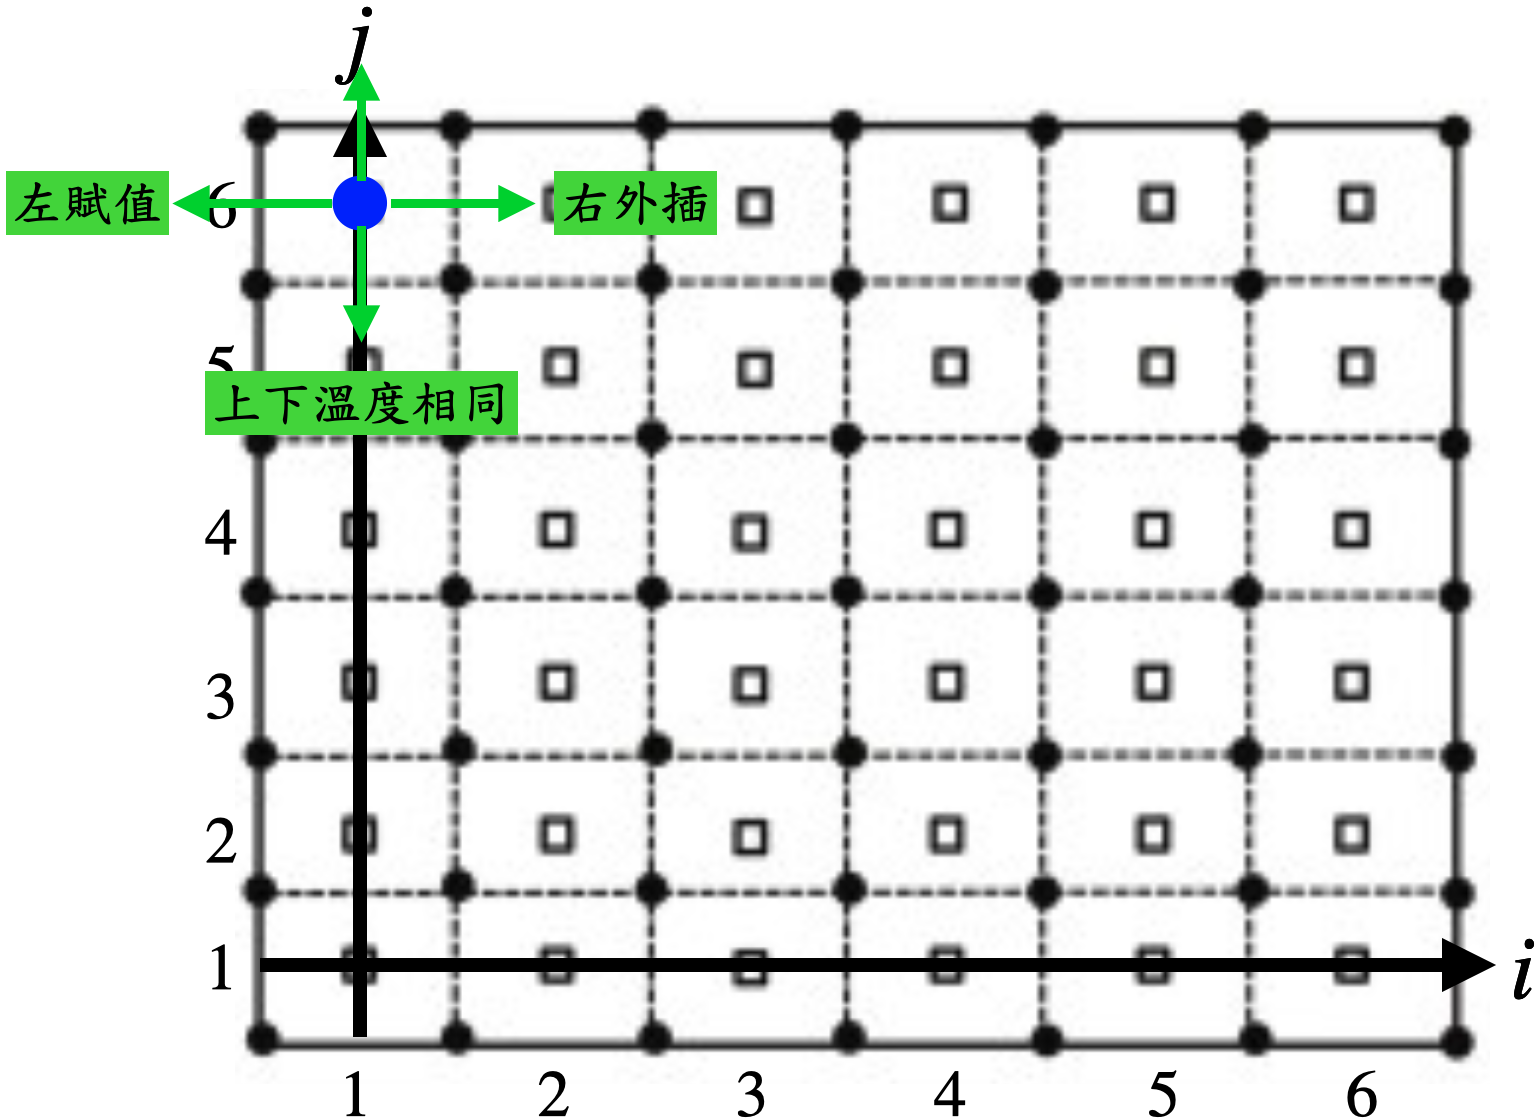
\includegraphics[width=\linewidth,height=9\baselineskip]{26.png}
   \label{fig:7th point}
\end{minipage}
\subsection{第八計算點}
 \begin{minipage}{0.6\textwidth}
   \noindent 範圍:$i=2\ ,\ j=N_{y}$\\[1.5ex]
   \noindent 邊界條件:$T_{left} = T_{-\frac{1}{2},N_{y}}= 1\ ,\ T_{up} = T_{1,N_{y}+\frac{1}{2}}=T_{1,N_{y}-\frac{1}{2}}$\\[1.5ex]
   \noindent 東西方向:採用式\eqref{eq:QUICK5}$\ ,\ $南北方向:採用式\eqref{eq:QUICK4}\\[1.5ex]
   \noindent 空間三階精度QUICK離散格式為:
   \begin{equation*}\begin{split}
   \Delta y(\frac{3}{8}T_{3,j} + \frac{3}{8}T_{2,j} -T_{1,j}) =\Delta y \frac{-2}{8}(T_{left}) \\[1.5ex]
   \end{split}\end{equation*}
   \end{minipage}                          
   \hfill
   \begin{minipage}{0.34\textwidth}
   \centering
   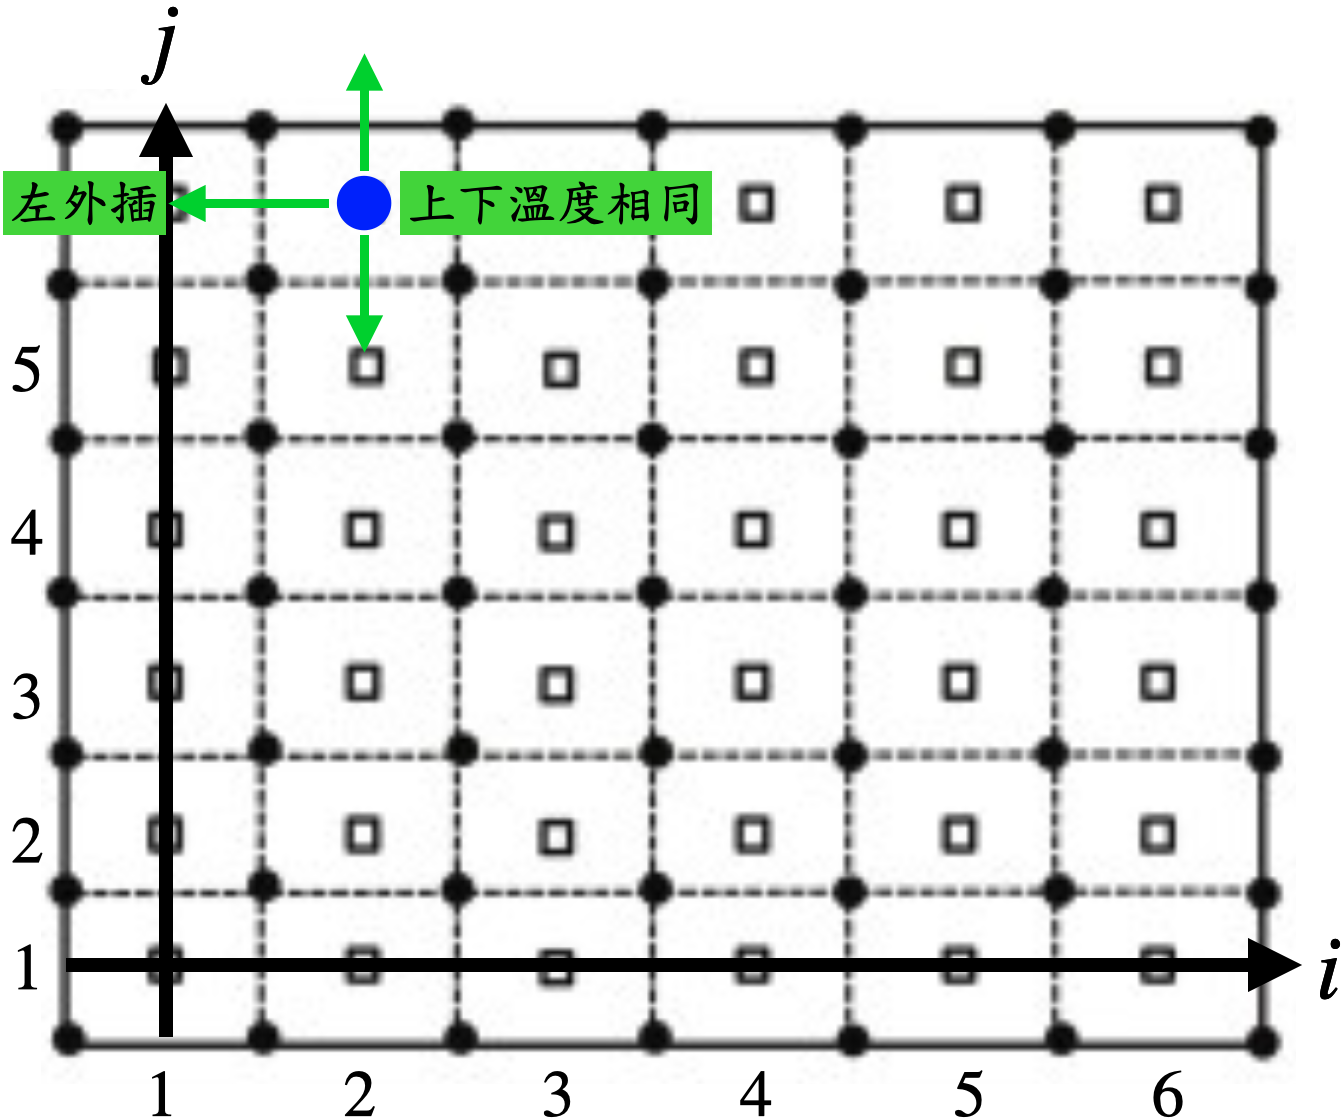
\includegraphics[width=\linewidth,height=9\baselineskip]{27.png}
   \label{fig:8th point}
\end{minipage}
\subsection{第九計算點}
 \begin{minipage}{0.6\textwidth}
   \noindent 範圍:$i=N_{x}\ ,\ j=N_{y}$\\[1.5ex]
   \noindent 邊界條件:$T_{right} = T_{N_{x}+\frac{1}{2},N_{y}}= 0\ ,\ T_{up} = T_{1,N_{y}+\frac{1}{2}}=T_{1,N_{y}-\frac{1}{2}}$\\[1.5ex]
   \noindent 東西方向:採用式\eqref{eq:QUICK2}$\ ,\ $南北方向:採用式\eqref{eq:QUICK4}\\[1.5ex]
   \noindent 空間三階精度QUICK離散格式為:
   \begin{equation*}\begin{split}
   -\Delta y(\frac{3}{8}T_{N_{x},j} + \frac{6}{8}T_{N_{x}-1,j} + \frac{-1}{8}T_{N_{x}-2,j}) = -\Delta y T_{right} \\[1.5ex]
   \end{split}\end{equation*}
   \end{minipage}%
   \hfill
   \begin{minipage}{0.34\textwidth}
   \centering
   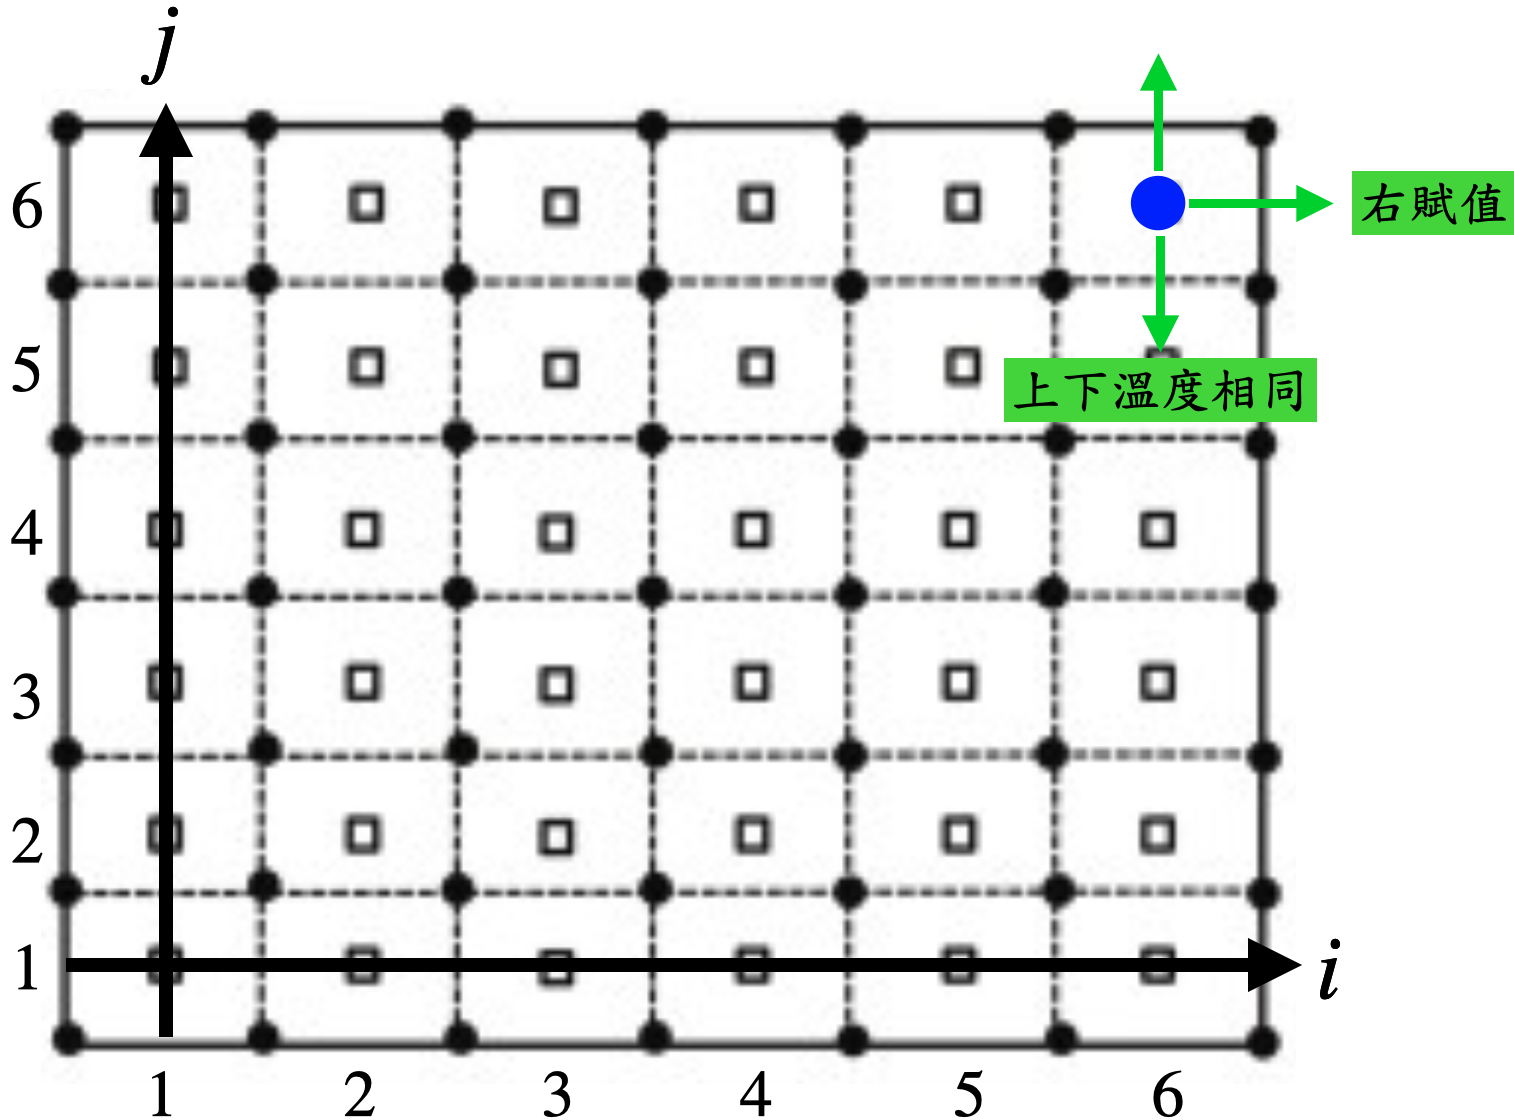
\includegraphics[width=\linewidth,height=9\baselineskip]{28.png}
   \label{fig:9th point}
\end{minipage}
\end{document}